\documentclass[aps,preprint,nofootinbib,floatfix]{revtex4-1}

\usepackage{amsmath,amssymb,amsfonts,amsthm,amscd,bm,bbm}
%\usepackage{nicefrac}       % compact symbols for 1/2, etc.
%\usepackage{microtype}      % microtypography
%\usepackage{mathtools}
%\usepackage{printlen}
%\usepackage{cite}
\usepackage[inline]{enumitem}
\usepackage[inline]{enumitem}
\usepackage[pdftex]{graphicx}
\graphicspath{{./figs/}}
\usepackage{algorithmic}
\usepackage{algorithm}
%\usepackage[none]{hyphenat}
\usepackage{multirow}
\usepackage{colortbl}
\usepackage{array,booktabs}
\usepackage{xcolor}
\usepackage{makecell}

%\pretolerance=10000
%\tolerance=2000 
%\emergencystretch=10pt

\newtheorem{theorem}{Theorem}
\newtheorem{definition}[theorem]{Definition}
\newtheorem{assumption}[theorem]{Assumption}
\newtheorem{lemma}[theorem]{Lemma}
\newtheorem{corollary}[theorem]{Corollary}
\newtheorem{proposition}[theorem]{Proposition}
\newtheorem{conjecture}[theorem]{Conjecture}
\newtheorem{remark}[theorem]{Remark}
\newtheorem{example}{Example}

\DeclareMathOperator{\aff}{aff}
\DeclareMathOperator{\st}{s.t.}
\DeclareMathOperator{\affnot}{aff_0}
\DeclareMathOperator{\conv}{conv}
\DeclareMathOperator{\relint}{relint}
\DeclareMathOperator{\vol}{vol}
\DeclareMathOperator{\range}{range}
\DeclareMathOperator{\image}{im}
\DeclareMathOperator{\nullspace}{null}
\DeclareMathOperator{\area}{area}
\DeclareMathOperator{\vspan}{span}
\DeclareMathOperator{\id}{Id}
\DeclareMathOperator{\cond}{cond}
\DeclareMathOperator{\prox}{prox}
\DeclareMathOperator*{\argmax}{arg\,max}
\DeclareMathOperator*{\argmin}{arg\,min}
\DeclareMathOperator*{\minimize}{minimize}
\DeclareMathOperator{\diag}{diag}
\DeclareMathOperator{\Tr}{Tr}

\newcommand\Energy{\mathcal{E}}
\newcommand\EnergyH{\mathcal{E}^{H}}
\newcommand\EnergyL{\mathcal{E}^{L}}
\newcommand\EnergyOne{\mathcal{E}^{1D}}
\newcommand\E{\mathbb{E}}
\newcommand\kk{K}
\newcommand\kkk{h}
\newcommand\Hk{{\mathcal{H}}_{\kk}}
\newcommand\HH{\mathcal{H}}
\newcommand\C{{\mathcal{C}}}
\newcommand\tC{{\widetilde{\C}}}
\newcommand\OO{{\mathcal{O}}}
\newcommand\Zt{Y}
\newcommand{\Ind}[1]{\mathbbm{1}_{#1}}
\newcommand\e{e}
\newcommand\om{\omega}


\begin{document}

\title{Energy Clustering}

\author{Guilherme Fran\c ca}
\email{guifranca@gmail.com} 
\author{Joshua T. Vogelstein}
\email{jovo@jhu.edu}
\affiliation{Johns Hopkins University}


\begin{abstract}
Energy statistics was proposed by Sz\' ekely in the 80's inspired by the 
Newtonian gravitational potential from classical mechanics, and it provides 
a hypothesis test for equality of distributions. Energy statistics was 
further generalized to data living metric spaces of strong negative type, 
and more recently a connection with reproducing kernel Hilbert spaces (RKHS) 
was proposed. Here we consider the problem of clustering data from an 
energy statistics 
theory perspective, called energy clustering for short, by providing a 
precise mathematical formulation yielding a quadratically constrained 
quadratic program (QCQP) in the associated RKHS, 
which we show to be equivalent to kernel $k$-means optimization problem.
Thus, our results imply a first principles derivation of kernel $k$-means 
from energy statistics.
Moreover, we also consider a weighted version of energy statistics 
applied to clustering, making connection to graph partitioning problems.
To find local optimizers of such QCQP we consider an iterative algorithm based 
on Hartigan's method, which in this case has the same computational cost 
as kernel $k$-means algorithm, based on Lloyd's method, but usually 
with better clustering quality. 
We provide carefully designed numerical experiments showing the superiority 
of the proposed method compared to kernel $k$-means, standard $k$-means, 
and gaussian mixture models in a variety of settings.
\end{abstract}

% @gui: have other people shown a relationship between kernel k-means and 
% say, RKHS, or something else? 
% @jovo: any kernel method is defined on a RKHS. 
% For instance ref [11] is the first one to consider kernel k-means in a 
% RKHS. The problem is how do you formulate a 
% statistical problem in a RKHS, or how do you know if there is a kernel
% related to it. In the case of energy statistics this was done by [6], and
% is a nontrivial result. It's based on this work that we have the theory 
% presented in this paper

\maketitle

%%%%%%%%%%%%%%%%%%%%%%%%%%%%%%%%%%%%%%%%%%%%%%%%%%%%%%%%%%%%%%%%%%%%%%%%%%%%%%%
\section{Introduction}

% @gui: algorithms don't make assumptions, theorems do.  also, algorithms cannot be parametric or non-parametric, that is a property only of the statistical model, or an estimator.

% @gui: k-means is NOT a special case of GMM, GMM is a soft clustering (not fuzzy, in stats and machine learning we don't say "fuzzy"), where as k-means is a hard clustering.  k-means is certainly closely related to GMM though.

% @gui:  don't know what "clear resolution of cluster centers" adds to this?

% @gui: algorithms cluster, doesn't matter how complicated the data are.  so, what do you actually mean here?  perform well empirically? what does "complicated" actually mean?

% @gui: the words "this" and "it" are often vague and ambiguous, be specific/precise

% @gui: not sure what you mean here, in kernel k-means, we don't "optimize" over any parameters typically.  sometimes we select hyperparameters of kernels via cross-validation, is that what you mean?

% @gui: not sure what you mean "only one possible optimization problem".  we can reformulate it many different ways? also, below, "this" is ambiguous.

% @gui: to me, we did not make explicit one of the most important points.   in this paper, we make clear exactly when we expect energy clustering to perform better than k-means/GMM, and when we expect it to perform worse (empirically).  

% @gui: i find ToC paragraphs useless.

% @jovo: corrected all of these points, and also re-wrote some other stuff. Please check. About ToC, I agree and wouldn't mind remove it, however it is a tradition that most referees like to see. In this case I included some important information about our work too, and it makes a transition between introduction and the remaining of the paper. If you want to remove it let me know and I will adapt.

Energy statistics \cite{Szkely2013}
is based on a 
notion of statistical potential energy between probability distributions,
in close analogy to Newton's gravitational potential in classical mechanics. 
It provides a hypothesis test for equality of distributions which is achieved 
under minimum energy. When probability distributions are different the 
statistical potential energy diverges as sample size increases, while tends 
to a nondegenerate limit distribution, i.e. remains finite, when they are 
equal. Energy statistics has been applied to several goodness-of-fit 
hypothesis tests, multi-sample tests of equality of distributions, 
analysis of variance \cite{RizzoVariance}, nonlinear dependence tests through
distance covariance and distance correlation, which generalizes the Pearson
correlation coefficient, and hierarchical clustering \cite{RizzoClustering} 
by extending Ward's method of minimum variance. Moreover, an application of 
energy statistics to clustering was already proposed \cite{Kgroups}, 
which in part motivated this paper. We refer the reader to \cite{Szkely2013}, 
and references therein, for an overview of energy statistics theory and 
its applications.

In its original formulation, energy statistics has a compact representation
in terms of expectations of pairwise Euclidean distances, providing
straightforward empirical estimates. 
The notion of distance covariance was further generalized from Euclidean 
spaces to metric spaces of strong negative type \cite{Lyons}. Moreover, 
the missing link between energy distance based tests and kernel based tests has 
been recently resolved \cite{Sejdinovic2013}, where a unifying framework
establishing an equivalence between generalized energy distances to maximum
mean discrepancies (MMD), which are distances between embeddings of 
distributions in reproducing kernel Hilbert spaces (RKHS), was established. 
This equivalence provides the link between energy distance based measures and 
RKHS based measures, commonly used in machine learning, and form the basis 
of our approach.

The clustering problem has such a long history in machine learning, making it
impossible to mention all important contributions in a short space. 
Perhaps, the most used method is $k$-means \cite{Lloyd,MacQueen,Forgy}, which
is based on Lloyd's heuristic \cite{Lloyd} of assigning a data point to
the cluster with closest center. The only statistical 
information about each cluster comes from its mean, and it is thus sensitive 
to outliers. Nevertheless, $k$-means works very well when data is 
linearly separable in Euclidean space. Gaussian mixture models (GMM) is also 
very commonly used for clustering, however, it makes strong assumptions about 
the distribution of the data, as $k$-means which is closely related to GMM. 

To account for nonlinearities, kernel methods were introduced 
\cite{Smola,Girolami}. A mercer kernel \cite{Mercer} is used to implicitly
map data points to a RKHS, then clustering can be performed in the associated
Hilbert space by using its inner product. Yet, the kernel choice remains 
the biggest challenge since there is no principled theory to construct a kernel
for a given dataset, and usually a kernel introduces hyperparameters that 
need to be carefully chosen.
The well-known kernel $k$-means optimization problem is nothing but $k$-means 
in the feature space \cite{Girolami}. Furthermore, kernel $k$-means algorithm
\cite{Dhillon2,Dhillon} is still based on Loyd's heuristic \cite{Lloyd} of
using the mean of each cluster in the feature space. 
We refer the reader to \cite{Filippone} for a survey of clustering
methods.

Although clustering from energy statistics was considered
in \cite{Kgroups}, the precise optimization problem behind this approach
remains elusive, as well as the connection to kernel methods.
The main theoretical contribution of this paper is to fill this gap.
Since the statistical potential energy is minimum when
distributions are equal, the principle behind clustering is to maximize 
the statistical energy,  enforcing probability distributions associated to 
each cluster to be different from one another. We provide a precise 
mathematical formulation to this statement, leading to a quadratically 
constrained quadratic program (QCQP) in the associated RKHS. Our results
immediately establish the connection to kernel methods, by showing that this 
QCQP is equivalent to kernel $k$-means optimization problem. The 
equivalence between kernel $k$-means, spectral clustering, and graph 
partitioning problems is well-known \cite{Dhillon,Dhillon2}. We demonstrate 
how these connections arise from a weighted version of energy statistics.

Our algorithmic contribution is to use Hartigan's method \cite{Hartigan} to 
find local solutions of the above mentioned QCQP, which is NP-hard in general.
Hartigan's method was also used in \cite{Kgroups}, and its advantages
over Lloyd's method was already being demonstrated \cite{Telgarsky,Slonin},
but apparently it did not receive the desired attention. To the 
best of our knowledge, Hartigan's method was not previously applied together 
with kernel methods. We provide an algorithm based on Hartigan's method in 
terms of the Gram matrix of the data computed from a kernel fixed by 
energy statistics. We make clear the advantages of this proposal versus 
Lloyd's method, which kernel $k$-means is based upon and will also be used 
to locally solve our QCQP. We show that both algorithms  have the same
time complexity. 

Our numerical results provide compelling evidence that 
Hartigan's method applied to energy statistics based clustering, 
or \emph{energy clustering} for short, is more accurate and robust than 
Lloyd's method. Moreover, in our experiments we put in evidence the
flexibility of energy clustering, which provides a family of default kernels, 
showing that it is able to perform accurately on data coming from 
very different distributions, contrary to $k$-means and GMM for instance.
More specifically, the proposed algorithms for energy clustering perform 
closely to $k$-means and GMM on normally distributed data. On the other
hand, it performs considerably better than $k$-means and GMM on  data that 
is not normally distributed. It also performs better than $k$-means 
and GMM in high dimensions, even on Gaussian settings. However, it performs 
worse than GMM, and more closely to $k$-means, for highly unbalanced clusters
with normal distributions.

Our work is organized as follows. In section~\ref{sec:background}, we introduce
the necessary background on energy statistics and RKHS.
Section~\ref{sec:clustering_theory} contains the main theoretical 
results of this paper,
where we consider a clustering theory based on energy statistics leading
to a QCQP, which is NP-hard in general. We also show the equivalence to 
kernel $k$-means optimization problem.
In Section~\ref{sec:weighted}, we generalize these results to a weighted
version of energy statistics, providing connections to graph
partitioning problems and spectral clustering.
In Section~\ref{sec:twoclass}, we consider the  simple case of a two-class
problem in one dimension,
where we propose an algorithm which requires no random initialization.
In section~\ref{sec:algo}, we consider Lloyd's and Hartigan's methods
and propose iterative algorithms to solve the QCQP.
Section~\ref{sec:numerics} contains some carefully designed numerical
experiments showing that in several settings, energy clustering based
on Hartigan's algorithm
outperms kernel $k$-means algorithm, standard $k$-means algorithm 
and GMM with the expectation maximization algorithm. 
Our final conclusions are presented in Section~\ref{sec:conclusion}.


%%%%%%%%%%%%%%%%%%%%%%%%%%%%%%%%%%%%%%%%%%%%%%%%%%%%%%%%%%%%%%%%%%%%%%%%%%%%%%%
\section{Background on Energy Statistics and RKHS}
\label{sec:background}

% @gui: i don't know what this means.  eqn 7 defines something for a population statistic, not a sample statistic.
% @jovo: removed. I was thinking that you can always estimate the expected 
% value by computing a sample mean. but I agree, it's confusing

% @gui: i'm not sure the above is true/meaningful.  nonparametric means implicitly estimating an infinite number of parameters.  without any statistical theory, i'm not quite sure what we can say.
% @jovo: I stoped saying non-parametric, however, Kolmogorov-Smirnov is also said to be non-parametric, so I thought that in this context it means that it does not assume any form of the distributions.

In this section we introduce the main concepts from energy
statistics and its relation to 
RKHS which form the basis of our work.
For more details we refer the reader
to \cite{Szkely2013} and \cite{Sejdinovic2013}.

Consider random variables in $\mathbb{R}^D$ 
such that $X,X' \stackrel{iid}{\sim} P$ and 
$Y,Y' \stackrel{iid}{\sim} Q$, where $P$ and $Q$ are cumulative
distribution functions with finite first moments. 
The quantity 
\begin{equation}
\label{eq:energy}
\Energy(P, Q) \equiv 2 \E \| X - Y\| - \E \| X - X' \| - \E \| Y - Y' \|,
\end{equation}
called \emph{energy distance} \cite{Szkely2013}, 
is rotationally invariant and nonnegative, $\Energy(P,Q) \ge 0$, where
equality
to zero holds if and only if $P = Q$.
Above, $\| \cdot \|$ denotes the
Euclidean norm in $\mathbb{R}^D$. 
Energy distance
provides a characterization of equality of distributions, and
$\Energy^{1/2}$ is
a metric on the space of distributions.

The energy distance can be generalized as, for instance,
\begin{equation}
\label{eq:energy2}
\Energy_\alpha(P, Q) \equiv 
2 \E \| X - Y\|^{\alpha} - \E \| X - X' \|^{\alpha} - 
\E \| Y - Y' \|^{\alpha}
\end{equation}
where $0<\alpha\le 2$. This quantity is also nonnegative,
$\Energy_\alpha(P,Q) \ge 0$. Furthermore, for $0<\alpha<2$ we have that
$\Energy_\alpha(P,Q) = 0$ if and only if $P=Q$, while for $\alpha=2$ 
we have $\Energy_2(P,Q) = 2\| \E(X) - \E(Y) \|^2$ which shows that
equality to zero only requires
equality of the means, and thus $\Energy_2(P,Q)=0$ does 
not imply equality of distributions.

The energy distance can be even further generalized.
Let $X, Y \in \mathcal{X}$  where $\mathcal{X}$ is an arbitrary space endowed
with a \emph{semimetric of negative type}
$\rho: \mathcal{X}\times\mathcal{X} \to \mathbb{R}$, which is required
to satisfy
\begin{equation}
\label{eq:negative_type}
\sum_{i,j=1}^n c_i c_j \rho(X_i, X_j) \le 0,
\end{equation}
where $X_i \in \mathcal{X}$ and $c_i \in \mathbb{R}$ such that
$\sum_{i=1}^n c_i = 0$. Then, $\mathcal{X}$ is called a \emph{space of
negative type}.
We can thus replace $\mathbb{R}^D \to \mathcal{X}$ and 
$\| X - Y \| \to \rho(X , Y)$ in the definition \eqref{eq:energy}, obtaining
the generalized energy distance
\begin{equation}
\label{eq:energy3}
\Energy(P, Q) \equiv 2 \E \rho(X,Y) - \E \rho(X, X') - \E \rho(Y,Y').
\end{equation}
For spaces of negative type there exists a Hilbert space $\mathcal{H}$ and
a map $\varphi: \mathcal{X} \to
\mathcal{H}$ such that
$\rho(X, Y) = \| \varphi(X) - \varphi(Y) \|_{\mathcal{H}}^2$. This
allows us to compute quantities related to probability distributions over
$\mathcal{X}$ in the Hilbert space $\mathcal{H}$.
Even though the semimetric 
$\rho$ may not satisfy the triangle inequality, 
$\rho^{1/2}$ does since it can be shown to be a proper metric. 

There is an equivalence between energy distance, 
commonly used in statistics,
and distances between embeddings of distributions in 
RKHS, commonly used in machine learning. 
This equivalence was established
in \cite{Sejdinovic2013}. Let us first recall the definition of
RKHS. Let $\HH$ be a Hilbert space of real-valued functions
over $\mathcal{X}$. A function 
$\kk : \mathcal{X} \times \mathcal{X} \to 
\mathbb{R}$ is a reproducing kernel of $\HH$ if it satisfies
the following two conditions:
\begin{enumerate}
\item $\kkk_x \equiv \kk(\cdot, x) \in \HH$ 
for all $x \in \mathcal{X}$.
\item $\langle \kkk_x, f \rangle_{\HH} = f(x)$ for
all $x\in\mathcal{X}$ and $f\in \HH$.
\end{enumerate}
In other words, for any $x \in \mathcal{X}$ and any function $f \in \HH$,
there is a unique 
$\kkk_x \in \HH$ that reproduces $f(x)$ through the inner product
of $\HH$.
If such a \emph{kernel} 
function $\kk$ exists, then $\HH$ is called a RKHS. The above two 
properties immediately imply that $\kk$ is symmetric and positive
definite. Indeed, notice that
$\langle \kkk_x, \kkk_y \rangle = \kkk_y(x) = \kk(x,y)$, and by 
definition 
$\langle \kkk_x, \kkk_y \rangle^* = \langle \kkk_y, \kkk_x \rangle$, but
since the inner product is real we have 
$\langle \kkk_y, \kkk_x \rangle = \langle \kkk_x, \kkk_y \rangle$, or
equivalently 
$\kk(y,x) = \kk(x,y)$. Moreover, for any $w \in
\HH$ we can write $w = \sum_{i=1}^n c_i \kkk_{x_i}$ where
$\{ \kkk_{x_i} \}_{i=1}^n$ is a basis of $\HH$. It follows that
$\langle w, w \rangle_{\HH}  = \sum_{i,j=1}^n c_i c_j \kk(x_i,x_j) \ge 0$,
showing that the kernel is positive definite. If $G$ is a matrix with
elements $G_{ij} = \kk(x_i,x_j)$ this is equivalent to $G$ being
positive semidefinite, i.e. $v^\top G \, v \ge 0$ for any vector
$v \in \mathbb{R}^n$.

The Moore-Aronszajn theorem 
\cite{Aronszajn}
establishes the converse of the above paragraph. 
For every symmetric
and positive definite function $\kk: \mathcal{X}\times \mathcal{X} \to
\mathbb{R}$, there is an associated RKHS $\Hk$ 
with reproducing
kernel $\kk$. The map $\varphi: x \mapsto \kkk_x \in \Hk$ is called
the canonical \emph{feature map}. Given a kernel $\kk$,
this theorem enables us to define an embedding of a probability measure
$P$ into the RKHS as follows: $P \mapsto \kkk_P \in
\Hk$ such that 
$\int f(x) d P(x) = \langle f, \kkk_P \rangle$ for all $f \in \Hk$,
or alternatively $\kkk_P \equiv \int \kk( \, \cdot \,, x)  d P(x)$. 
We can now  introduce the 
notion of distance between two probability measures using the inner product
of $\Hk$, which is called the maximum mean discrepancy (MMD) and
is given by
\begin{equation}
\label{eq:mmd}
\gamma_\kk(P,Q) \equiv \| \kkk_P - \kkk_Q \|_{\Hk}.
\end{equation}
This can also be written as \cite{Gretton2012}
\begin{equation}\label{eq:mmd2}
\gamma_\kk^2(P,Q) = \E \kk(X,X') + \E \kk(Y,Y') - 2 \E \kk(X, Y)
\end{equation}
where $X,X' \stackrel{iid}{\sim} P$ and $Y,Y'\stackrel{iid}{\sim} Q$.
From the equality between \eqref{eq:mmd} and \eqref{eq:mmd2} we also
have 
\begin{equation}\label{eq:inner_data}
\langle \kkk_P, \kkk_Q \rangle_{\Hk} = \E \, \kk(X, Y).
\end{equation}
Thus, in practice, we can estimate the inner product between  
embedded distributions 
by averaging the kernel function over sampled data.

The following important result shows that semimetrics of negative
type and symmetric positive definite kernels are closely related
\cite{Berg1984}. Let $\rho: \mathcal{X} \times \mathcal{X} \to \mathbb{R}$
and $x_0 \in \mathcal{X}$ an arbitrary but fixed point.
Define
\begin{equation}
\label{eq:kernel_semimetric}
\kk(x,y) \equiv 
\tfrac{1}{2} \left[  \rho(x,x_0) + \rho(y,x_0) - \rho(x,y)\right].
\end{equation}
Then, it can be shown that 
$\kk$ is positive definite if and only if $\rho$ is a semimetric
of negative type.
We have a family of kernels, one for each choice of $x_0$. Conversely,
if $\rho$ is a semimetric of negative type and $\kk$ is a kernel in this
family, then 
\begin{equation}
\label{eq:gen_kernel}
\begin{split}
\rho(x,y) &= \kk(x,x) + \kk(y,y) -2\kk(x,y) \\
&=  \| \kkk_x - \kkk_y \|^2_{\Hk}
\end{split}
\end{equation}
and the canonical feature map 
$\varphi: x \mapsto \kkk_x$ is injective \cite{Sejdinovic2013}.
When these conditions are satisfied we say that the kernel $\kk$ 
generates the semimetric $\rho$. 
If two different kernels generate the same $\rho$ they are
equivalent kernels.

Now we can state the equivalence between energy distance $\Energy$ and
inner products on RKHS, which is one of the main results of
\cite{Sejdinovic2013}. If $\rho$ is a semimetric
of negative type and $\kk$ a kernel that generates $\rho$, then
replacing \eqref{eq:gen_kernel} into
\eqref{eq:energy3}, and using \eqref{eq:mmd2}, yields
\begin{equation} \label{eq:Erho}
\Energy(P, Q) = 
2 \left[ \E \, \kk(X, X') + \E \, \kk(Y, Y') - 2\E \, \kk(X, Y)\right] 
= 2 \gamma_\kk^2(P,Q) .
\end{equation}
Due to \eqref{eq:mmd} we can compute the energy distance using the inner 
product of $\Hk$. 

Finally, let us recall the main formulas from energy statistics
for the test statistic of equality of distributions \cite{Szkely2013}. 
Assume we have data $\mathbb{X} = \{ x_1,\dotsc, x_n \}$ where
$x_i \in \mathcal{X}$, and $\mathcal{X}$ is a space of negative type.
Consider a disjoint partition $\mathbb{X} = \bigcup_{j=1}^k \C_j$, with
$\C_i \cap \C_j = \emptyset$.
Each expectation in the generalized energy distance
\eqref{eq:energy3}
can be computed 
through the function
\begin{equation}
\label{eq:g_def}
g (\C_i, \C_j) \equiv 
\dfrac{1}{n_i n_j}
\sum_{x \in \C_i} 
\sum_{y \in \C_j} \rho(x, y)
\end{equation}
where $n_i = |\C_i|$ is the number of elements in partition
$\C_i$. 
The \emph{within energy dispersion} is defined by
\begin{equation}
\label{eq:within}
W \equiv
\sum_{j=1}^{k} \dfrac{n_j}{2} g(\C_j, \C_j),
\end{equation}
and the \emph{between-sample energy statistic} is defined by
\begin{equation}
\label{eq:between}
S \equiv
\sum_{1 \le  i < j \le k } \dfrac{n_i n_{j}}{2 n} \left[
2 g(\C_i, \C_j) - 
g(\C_i, \C_i) - 
g(\C_j, \C_j)
\right],
\end{equation}
where $n = \sum_{j=1}^k n_j$.
Given a set of distributions
$\{ P_j\}_{j=1}^k$, where $x \in \C_j$ if and only if $x \sim P_j$, 
the quantity $S$ provides
a test statistic for equality of distributions
\cite{Szkely2013}.
When the sample size is large enough, $n\to \infty$,
under the null hypothesis $H_0: P_1=P_2=\dotsm=P_k$ we have that
$S\to 0$, 
and under
the alternative hypothesis $H_1: P_i \ne P_j$ for at least two $i\ne j$, 
we have that $S \to \infty$.
This test does not make any assumptions
about the distributions $P_j$.

One can make a physical analogy by thinking 
that points $ x \in \C_j$ form a massive body 
whose total mass is characterized by the distribution function $P_j$.
The quantity $S$ is thus a potential
energy of the from $S(P_1,\dotsc,P_k)$ which measures how different
the distribution of these masses are,  and achieves the ground state
$S=0$ when all bodies have the same mass distribution. The potential energy
$S$ increases as bodies have different mass distributions.


%%%%%%%%%%%%%%%%%%%%%%%%%%%%%%%%%%%%%%%%%%%%%%%%%%%%%%%%%%%%%%%%%%%%%%%%%%%%%%%
\section{Clustering Based on Energy Statistics}
\label{sec:clustering_theory}

% @gui: consider only using equation numbers for equations that you later refer to? there are so many, it is easy to get lost.
% @jovo: ok, will do that after we finish everything. There is a package that automatically remove numbers from unreferenced equations

% @gui: where possible, i recommend using the "name" of the quantity rather than the number of the equation.  eg, here, write S and W, rather than (13) and (12).
% @jovo: ok, I will do that for the main symbols, and refer to equations only when necessary

% @gui: do other people know this result? (about min W = max X) if so, cite them, if not, state that.
% @jovo: eq (15), i.e. S + W = T is well-known. Gabor and Rizzo wrote that
% in their paper, however, they didn't write a proof. They should have
% it in some other paper.  However, they mention 
% that this holds only for 0 < alpha < 2, with |x-y|^alpha, while
% here I did for a general semimetric. The PhD thesis do not 
% mention anywhere that minimizing W is equivalent to maximizing S.
% Thus, although a trivial result, but important, I didn't see this 
% written explicitly before.

% @gui: "Let us" is used a bunch, though i think it never adds anything? i'd remove it everywhere.
% @jovo: ok, remove it all along

% @gui: i don't understand the notaiton (.)_jj. is a sum missing?
% @jovo: this is standard.  A_{ij} denotes the 
% $(i,j)$th element of matrix A as you know. 
% Since here A = Z^T G Z is a product of 3 matrices
% we just put a parenthesis to avoid confusion, that's all

% @gui: don't use equation numbers here.
% @jovo: in some cases it is unavoidable. I tried to do that when the context
% is obvious, by writing the symbols, but when we refer to long 
% expressions or derivation steps it is way more clear so say, replace equation (1) into (2) to get ... than saying, replacing A into B to get ... and the reader has to glance through the entire paper to recall what A and B are.

% @gui: this might be a better initialization than k-means++, which essentially initializes using a different kernel?
% @jovo: yes it might be, and I agree, k-means++ is initializing in "Euclidean
% space" not in the feature space where data might be better separable. We will do this from now on.

% @gui: i'm not sure about this.  who is to say the correct direction of causality? maybe energy clustering is a special case of kernel k-means?
% @jovo: tried to not commit to a single view. We show that they are
% equivalent, when opperating on the same kernel. However, kernel k-means per
% se does not consider anything about the kernel choice. Energy statistics,
% however, provides a theory valid on spaces of negative type, which guarantees
% that a kernel constructed in this formalism will be positive-semidefinite.

In this vein, kernel $k$-means is part of a
This section contains the main theoretical results of this paper, where 
we formulate an optimization problem for clustering 
based on energy statistics and RKHS introduced in the previous section.

Due to the energy test statistic for equality of distributions,
the obvious
criterion for clustering data is to 
maximize $S$ which makes 
each cluster as different
as possible from the other ones.
In other words, given a set of points coming from different probability
distributions, $S$ should attain a maximum when each point is correctly
classified as belonging to the cluster associated to its probability
distribution.
The following 
straightforward result
shows that maximizing $S$ is, however, equivalent to minimizing
$W$ which has a more convenient form.

\begin{proposition}
\label{th:minimize}
Let $\mathbb{X} = \{x_1,\dotsc,x_n\}$ where each data point
$x_i$ lives in a space $\mathcal{X}$ endowed with a semimetric $\rho:
\mathcal{X}\times\mathcal{X} \to \mathbb{R}$ of
negative type. For a fixed integer $k$,
the partition
$\mathbb{X} = \bigcup_{j=1}^k \C_j$, where $\C_i \cap C_j = \emptyset$ for
all $i\ne j$, maximizes the between-sample statistic $S$, defined
in equation \eqref{eq:between}, if and only if
\begin{equation}
\label{eq:minimize}
\min_{\C_1,\dotsc,C_k  } W(
\C_1, \dotsc, \C_k),
\end{equation}
where the within energy dispersion $W$ is defined by \eqref{eq:within}.
\end{proposition}
\begin{proof}
From \eqref{eq:within} and \eqref{eq:between}
we have
\begin{equation}
\begin{split}
S + W &= 
\dfrac{1}{2n} \sum_{\substack{i,j=1 \\ i\ne j}}^k n_i n_j g(\C_i, \C_j)
+ \dfrac{1}{2n} \sum_{i=1}^{k} 
\bigg[ n - 
\sum_{j\ne i = 1}^k n_j \bigg] 
n_i g(\C_i, \C_i) \\
& = \dfrac{1}{2n} \sum_{i,j=1}^k n_i n_j g(\C_i, \C_j)
= \dfrac{1}{2n} \sum_{x \in \mathbb{X}} \sum_{y \in \mathbb{X}} \rho(x,y)
= \dfrac{n}{2} g(\mathbb{X}, \mathbb{X}).
\end{split}
\end{equation}
Note that the right hand side of this equation 
only depends on the pooled data, so it is a constant
independent of the choice of partition. Therefore, maximizing
$S$ over the choice of partition is equivalent to minimizing $W$.
\end{proof}

For a given $k$, the clustering problem amounts to
finding the best partition of the data by minimizing $W$.
Notice that this is a hard clustering problem as partitions
are disjoint. The optimization problem \eqref{eq:minimize} based on
energy statistics was already proposed in \cite{Kgroups}. However, it is
important to note that this is equivalent to maximizing $S$
which is the test statistic for equality of distributions. In this current
form, the relation with kernels and to other clustering methods is obscure.
In the following, we show what is the explicit optimization problem behind 
in the corresponding RKHS, establishing the connection to kernel methods.

We now formulate the analog of the optimization problem \eqref{eq:minimize} 
in the corresponding RKHS. 
Based on the relation between kernels and semimetrics, see 
\eqref{eq:kernel_semimetric} and \eqref{eq:gen_kernel}, 
assume that the kernel $\kk: \mathcal{X} \times \mathcal{X} \to \mathbb{R}$ 
generates $\rho$.  Define  the Gram matrix
\begin{equation}
\label{eq:kernel_matrix}
G \equiv \begin{pmatrix}
\kk(x_1,x_1) & \kk(x_1,x_2) & \dotsm & \kk(x_1,x_n) \\
\kk(x_2,x_1) & \kk(x_2,x_2) & \dotsm & \kk(x_2,x_n) \\
\vdots & \vdots & \ddots  & \vdots \\
\kk(x_n,x_1) & \kk(x_n,x_2) & \dotsm & \kk(x_n,x_n) 
\end{pmatrix} .
\end{equation}
Let $Z \in \{ 0,1 \}^{n\times k}$ be the label matrix, 
with only one nonvanishing entry per row, 
indicating to which cluster (column)
each point (row) belongs to. This matrix satisfies
$Z^\top Z = D$, where the diagonal matrix 
$D = \diag( n_1,\dotsc, n_k )$  contains
the number of points in each cluster. We also introduce the rescaled
matrix  $Y \equiv Z D^{-1/2}$. In component form they are given by
\begin{equation}
\label{eq:label_matrix}
Z_{ij} \equiv \begin{cases}
1 & \mbox{if $x_i \in \C_j$ } \\
0 & \mbox{otherwise}
\end{cases} \qquad
\Zt_{ij} \equiv \begin{cases}
\tfrac{1}{\sqrt{n_j}} & \mbox{if $x_i \in \C_j$ } \\
0 & \mbox{otherwise}
\end{cases} .
\end{equation}
Throughout the paper, we use the notation $M_{i\bullet}$ to denote
the $i$th row of a matrix $M$, and $M_{\bullet j}$ denotes its $j$th column.
Our next result shows that the optimization problem \eqref{eq:minimize}
is NP-hard since
it is a quadratically constrained quadratic program (QCQP) in the RKHS.

\begin{proposition} 
\label{th:qcqp2}
The optimization problem \eqref{eq:minimize} is equivalent to
\begin{equation}
\label{eq:qcqp2}
\max_{\Zt} \Tr \left( \Zt^\top G \, \Zt \right)  \qquad
\mbox{s.t. $\Zt \ge 0$, $\Zt^\top \Zt = I$, 
$\Zt \Zt^\top \e = \e$},
\end{equation}
where $\e = (1,1,\dots,1)^\top \in \mathbb{R}^n$ is the all-ones vector,
and $G$ is the Gram matrix \eqref{eq:kernel_matrix}.
\end{proposition}
\begin{proof}
From 
\eqref{eq:gen_kernel},
\eqref{eq:g_def}, and
\eqref{eq:within}
we have
\begin{equation}
\label{eq:W2}
W(\C_1,\dotsc,\C_k  )
= \dfrac{1}{2} \sum_{j=1}^k \dfrac{1}{n_j} \sum_{x,y \in \C_j} \rho(x,y)
= \sum_{j=1}^k \sum_{x \in \C_j}  \bigg(
\kk(x,x) - \dfrac{1}{n_j} \sum_{y \in \C_j} \kk(x,y) \bigg).
\end{equation}
Note that the first term is global so it does not contribute to the 
optimization problem.
Therefore, minimizing \eqref{eq:W2} is equivalent to
\begin{equation}
\label{eq:max_prob}
\max_{ \C_1,\dotsc,\C_k } 
\sum_{j=1}^k \dfrac{1}{n_j} \sum_{x,y\in C_j} \kk(x,y) .
\end{equation}
But 
\begin{equation}
\sum_{x, y \in \C_j} \kk(x, y) =
\sum_{p=1}^{n} \sum_{q=1}^{n} Z_{pj} Z_{qj} G_{pq} = 
(Z^\top G \, Z)_{jj},
\end{equation}
where we used the definitions \eqref{eq:kernel_matrix} and
\eqref{eq:label_matrix}. Thus, the objective function in 
\eqref{eq:max_prob} is equal to
$\Tr \left( D^{-1} Z^\top G Z \right)$. 
% @gui: the above step is not obvious
% @jovo: It is obvious. 
% From (21) we have \sum_j 1/n_j (Z^T G Z)_jj. But 1/n_j is just
% D^{-1}_jj (the diagonal matrix). The sum over j goes over the diagonals of
% D^{-1} Z^T G Z which is the definition of the trace
Now we can
use the cyclic property
of the trace, and by the  definition of the matrix $Z$
in \eqref{eq:label_matrix}, we obtain the following integer
programing problem:
\begin{equation}\label{eq:qcqp}
\max_{Z} \Tr\Big( \big( Z D^{-1/2}\big)^\top G 
\big( ZD^{-1/2} \big) 
\Big) \quad
\mbox{s.t. $Z_{ij} \in \{0,1\}$, $\sum_{j=1}^k Z_{ij} = 1$, 
$\sum_{i=1}^n Z_{ij} = n_j$.}
\end{equation}

Now we write this in terms of the matrix $Y = Z D^{-1/2}$.
The objective function immediately becomes
$\Tr\left( Y^\top G \, Y\right)$. Notice that the above constraints
imply that $Z^T Z = D$, where $D=\diag(n_1,\dotsc,n_k)$, which in turn gives
$D^{-1/2} Y^T Y D^{-1/2} = D$, or $Y^\top Y = I$. 
Also, every entry of $Y$ is positive by definition,
$Y \ge 0$. Now it only remains to show the last 
constraint in \eqref{eq:qcqp2}, which comes from the last
constraint in \eqref{eq:qcqp}. In matrix form this reads
$Z^T \e = D \e$. Replacing $Z=YD^{1/2}$ we have
$Y^\top \e = D^{1/2} \e$. Multiplying this last equation
on the left by $Y$, and noticing
that $Y D^{1/2} \e = Z \e = \e$, we finally obtain
$Y Y^\top \e = \e$. Therefore, the optimization 
problem \eqref{eq:qcqp} is equivalent
to \eqref{eq:qcqp2} .
\end{proof}

Based on Proposition~\ref{th:qcqp2}, to group data
$\mathbb{X} = \{ x_1,\dotsc,x_n \}$
into  $k$ clusters we first compute the Gram matrix
$G$ and then 
solve the optimization problem \eqref{eq:qcqp2} for $\Zt \in
\mathbb{R}^{n\times k}$. The $i$th row
of $\Zt$ will contain a single nonzero element in some $j$th column,
indicating that $x_i \in \C_j$. 
This optimization problem is nonconvex, and also NP-hard,
thus a direct approach 
is computational prohibitive even for small datasets.
However, one can find approximate solutions by relaxing some 
of the constraints, or obtaining a relaxed SDP version of it.
For instance, the relaxed problem
\begin{equation}
\label{eq:relaxed}
\max_{Y} \Tr \left( Y^\top G \, Y \right) \quad \mbox{s.t. $Y^\top Y = I$}
\end{equation}
has a well-known closed form solution $Y^\star = U R$, where the
columns of $U \in \mathbb{R}^{n\times k}$ 
contain the top $k$ eigenvectors of $G$ corresponding
to the $k$ largest eigenvalues $\lambda_1\ge \lambda_2\ge\dotsc\ge\lambda_k$, 
and
$R \in \mathbb{R}^{k\times k}$ is an arbitrary orthogonal matrix. 
The resulting
optimal objective function value is thus
$\max \Tr \left( {Y^\star}^\top G \, Y^\star \right)  = 
\sum_{i=1}^k \lambda_i$. 

Spectral clustering is based on the above approach, where
one further normalize the rows of $Y^\star$, 
i.e. $Y^\star \to \widetilde{Y}$ where 
$\widetilde{Y}_{ij} \equiv Y^\star_{ij}/ \| Y^\star_{i\bullet} \|$. 
The vectors
$y_i \equiv \widetilde{Y}_{i\bullet} \in \mathbb{R}^k$, which are the
rows of matrix $\widetilde{Y}$, lie on the surface of the $k$-dimensional 
unit sphere.
The set $\{ y_i \}_{i=1}^n$ is a spectral embedding of the original
set $\{ x_i \}_{i=1}^n$ onto an eigen-subspace of the kernel matrix $G$.
One then group the points $\{ y_i \}_{i=1}^n$ into $k$ clusters 
$\{ \tC_1,\dotsc,\tC_k \}$, using any clustering algorithm such as
$k$-means, yielding the final solution
where the original point $x_i$ belongs
to cluster $\C_j$ if and only if $y_i$ belongs to $\tC_j$.
A procedure on these lines was proposed in the seminal paper
\cite{NgJordan}, which considers the eigen-decomposition of
the matrix $D^{-1/2} G D^{-1/2}$ instead of $G$, and also 
where $G$ is an affinity matrix with the 
modification that its diagonal elements are set to zero $G_{ii}=0$, 
and $D=\diag(d_{1},\dotsc,d_{n})$ is the degree matrix, 
$d_{i} \equiv \sum_{j=1}^n G_{ij}$. 
Here we consider a slightly different
prescription which we call $\mathcal{E}$-spectral, using exactly the same 
approach, but considering the
eigen-decomposition of $G D^{-1}$ instead\footnote{
We found empirically that our method is more stable and often more
accurate than \cite{NgJordan}.}. Our method is described in 
Algorithm~\ref{spectralalgo}, and will be used as an initialization to the
iterative algorithms to solve the full optimization problem \eqref{eq:qcqp2}
that will be proposed later.

\begin{figure}
\begin{flushleft}
\begin{algorithm}[H]
\vspace{.5em}
\begin{algorithmic}[1]
\INPUT Gram matrix $G\in\mathbb{R}^{n\times n}$, and number of clusters $k$
\OUTPUT label matrix $Z \in \{ 0, 1\}^{n \times k}$
\STATE set the diagonal of $G$ to zero: $G_{ii} \leftarrow 0$ 
        for $i=1,\dotsc,n$
\STATE $D\leftarrow\diag(d_1,\dotsc,d_n)$ 
        where $d_i \leftarrow \sum_{j=1}^n G_{ij}$
\STATE solve the generalized eigenvalue problem $G v_i = \lambda_i D v_i$,
        where $i=1,\dotsc,n$ with eigenvalues, and corresponding eigenvectors,
        obeying the ordering
        $\lambda_1 \ge \lambda_2 \ge \dotsc \lambda_n$
\STATE $Y \leftarrow (D v_1| \dotsm | D v_k) 
        \in \mathbb{R}^{n\times k}$ 
has the top $k$ eigenvectors (multiplied by $D$) as columns
\STATE normalize the rows $Y$, i.e. $\widetilde{Y}_{ij} \leftarrow Y_{ij} / 
\left(\sum_{j=1}^n |Y_{ij}|^2\right)^{1/2}$
\STATE apply $k$-means on $\{ y_i \}_{i=1}^n$, 
where $y_i = \widetilde{Y}_{i\bullet}$
is the $i$th row of $\widetilde{Y}$
\STATE $Z_{ij} \leftarrow 1$ if $y_i$ is in cluster $j$, 
        and $Z_{ij} \leftarrow 0$ otherwise
\end{algorithmic}
\caption{
\label{spectralalgo}
$\mathcal{E}$-spectral is an exact method to solve
the relaxed problem \eqref{eq:relaxed}.
\hspace{\fill}
}
\end{algorithm}
\end{flushleft}
\end{figure}

Note that the energy clustering problem \eqref{eq:qcqp2} 
is valid for data living in an \emph{arbitrary} space of negative type where
a semimetric $\rho$, and thus the kernel $\kk$, are
assumed to be known. For instance, standard energy statistics in
Euclidean space fixes a family of choices, 
$\rho(x,y) = \| x - y\|^\alpha$ and the corresponding
kernel $K(x,y) = \tfrac{1}{2} \left( \| x \|^\alpha + \| y \|^\alpha - 
\| x-y\|^\alpha \right)$, where we
set $x_0=0$ in \eqref{eq:kernel_semimetric}, for $0<\alpha\le 2$.
For data living in a more general
metric space $(\mathcal{X}, \rho)$ the corresponding semimetric $\rho$ fixes
the kernel.
In any case, the energy  clustering 
formulation does not make assumptions
about  the distribution of the data, 
contrary to $k$-means and GMM, for example.
In practice, however,
the clustering quality strongly depend on the choice of a suitable
$\rho$, which measures the similarity between data points,
and is equivalent to choosing an appropriate kernel.
However, if prior information is available to choose a suitable $\rho$,
the energy clustering conviniently incorporate this measure in the 
optimization problem \eqref{eq:qcqp2}.


\subsection*{Relation to Kernel $\bm{k}$-Means}

One may wonder how energy clustering 
relates to the well-known kernel $k$-means problem%
\footnote{When we refer to kernel $k$-means problem we mean specifically 
the optimization problem \eqref{eq:kernel_kmeans}, which should not be 
confused with kernel $k$-means algorithm that is just one possible recipe 
to solve \eqref{eq:kernel_kmeans}.} 
which is extensively used in machine learning.
For a positive semidefinite Gram matrix $G$, as defined in
\eqref{eq:kernel_matrix},
there exists a map
$\varphi: \mathcal{X} \to \HH_\kk$ such that
$\kk(x,y) = \varphi(x)^\top \varphi(y)$. The kernel $k$-means optimization
problem,
in feature space,
is defined by
\begin{equation}
\label{eq:kernel_kmeans}
\min_{\C_1,\dotsc,\C_k}\bigg\{ 
J(\C_1,\dots,\C_k) \equiv  \sum_{j=1}^k
\sum_{x \in \C_j} \| \varphi(x) - \varphi(\mu_j) \|^2
\bigg\}
\end{equation}
where $\mu_j = \tfrac{1}{n_j} \sum_{x \in \C_j} x$ is the  mean of cluster
$\C_j$ in the ambient space. Notice that the above objective function
is strongly tied to the idea of minimizing distances between points
and cluster centers, which arises from $k$-means objective function based
on Lloyd's method \cite{Lloyd}.
It is known \cite{Dhillon2,Dhillon}
that problem \eqref{eq:kernel_kmeans} 
can be cast into a trace maximization problem in the same form as 
\eqref{eq:qcqp2}. The next result makes this explicit, showing that
\eqref{eq:minimize} and \eqref{eq:kernel_kmeans} are actually equivalent.

\begin{proposition}
\label{th:kernel_kmeans}
For a fixed kernel,
the clustering optimization problem
\eqref{eq:minimize} based on energy statistics 
is equivalent to the kernel $k$-means optimization problem
\eqref{eq:kernel_kmeans}, and both are equivalent to \eqref{eq:qcqp2}.
\end{proposition}
\begin{proof}
Notice that $\| \varphi(x) - \varphi(\mu_j) \|^2 = \varphi(x)^\top \varphi(x)
- 2 \varphi(x)^\top \varphi(\mu_j) + \varphi(\mu_j)^\top \varphi(\mu_j)$,
therefore
\begin{equation}
\label{eq:J}
J = \sum_{j=1}^k \sum_{x\in\C_j} \bigg(
\kk(x,x) - 
\dfrac{2}{n_j} \sum_{y\in \C_j} \kk(x,y) + \dfrac{1}{n_j^2}
\sum_{y,z \in \C_j} \kk(y,z) \bigg).
\end{equation}
The first term is global so it does not contribute to the optimization
problem. Notice that the third term gives
$\sum_{x\in\C_j} \tfrac{1}{n_j^2} \sum_{y,z\in\C_j} \kk(y,z) =
\tfrac{1}{n_j}\sum_{y,z\in\C_j} \kk(y,z)$, which is the same as
the second term. Thus, problem
\eqref{eq:kernel_kmeans} is equivalent to
\begin{equation}
\max_{\C_1,\dotsc,\C_k}
\sum_{j=1}^k \dfrac{1}{n_j} \sum_{x,y \in\C_j} \kk(x,y) 
\end{equation}
which is exactly the same as 
\eqref{eq:max_prob} from the energy statistics formulation. Therefore,
once the kernel $\kk$ is fixed, the function 
$W$ given by \eqref{eq:within} is the same
as $J$ in \eqref{eq:kernel_kmeans}.
The remaining of the proof proceeds as 
already shown in the proof of Proposition~\ref{th:qcqp2}, leading to
the optimization problem \eqref{eq:qcqp2}.
\end{proof}

The above result shows that 
kernel $k$-means problem is equivalent to the clustering problem
formulated in the energy statistics framework, when operating on the same
kernel. Notice, however, that 
energy statistics theory is valid for arbitrary semimetric spaces of
negative type, and the corresponding kernel in the associated RKHS is
guaranteed to be positive semi-definite.

As shown in \cite{Dhillon2,Dhillon}, kernel $k$-means, spectral clustering,
and graph partitioning problems such as ratio association, ratio cut, and
normalized cut are all equivalent to a QCQP of the form \eqref{eq:qcqp2}. Thus
one can use kernel $k$-means algorithm to solve these problems as well.
This correspondence involves a weighted version of problem 
\eqref{eq:qcqp2}, that
we demonstrate in the following from the perspective of energy statistics.


%%%%%%%%%%%%%%%%%%%%%%%%%%%%%%%%%%%%%%%%%%%%%%%%%%%%%%%%%%%%%%%%%%%%%%%%%%%%%%%
\section{Clustering Based on Weighted Energy Statistics}
\label{sec:weighted}

We generalize the formulas from energy statistics to incorporate
weights associated to each data point.
Let $w(x)$ be a weight function associated to point $x \in \mathcal{X}$.
We can generalize \eqref{eq:g_def} as follows:
\begin{equation}
\label{eq:g_def2}
g(\C_i, \C_j) \equiv \dfrac{1}{s_i s_j} \sum_{x\in \C_i}\sum_{y\in\C_j}
w(x)w(y) \rho(x,y), \qquad s_i \equiv \sum_{x\in\C_i} w(x).
\end{equation}
Now we replace this function in the formulas \eqref{eq:within} and
\eqref{eq:between}, with 
$n_i \to s_i$ and $n \to s$ where $s = \sum_{j=1}^k s_j$,
to obtain a weighted version of energy test statistic. With these
changes, Proposition~\ref{th:minimize} remains the unaltered, so the
clustering problem becomes
\begin{equation}
\label{eq:minimize2}
\min_{\C_1, \dotsc, \C_k} 
\bigg\{
W(\C_1,\dotsc,\C_k) \equiv \sum_{j=1}^k \dfrac{s_j}{2} g(\C_j,\C_j)
\bigg\}
\end{equation}
where now $g$ is given by \eqref{eq:g_def2}. 
Let us define the following matrices and vector:
\begin{equation}
\label{eq:weighted_matrices}
Y_{ij} \equiv \begin{cases}
\tfrac{1}{\sqrt{s_j}} & \mbox{if $x_i \in \C_j$} \\
0 & \mbox{otherwise}
\end{cases}, \qquad
\mathcal{W} \equiv \diag(w_1,\dotsc,w_n), \qquad
H \equiv \mathcal{W}^{1/2} Y, \qquad
\om \equiv \mathcal{W} \e,
\end{equation}
where $w_i = w(x_i)$ and $\e \in \mathbb{R}^n$ is the all-ones
vector. Now we can show the analogous of
Proposition~\ref{th:qcqp2} to the case of problem \eqref{eq:minimize2}.

\begin{proposition}
\label{th:qcqp3}
The weighted version of energy statistics clustering given by
problem \eqref{eq:minimize2} is equivalent to
\begin{equation}
\label{eq:qcqp3}
\max_H \Tr \left\{ H^\top (\mathcal{W}^{1/2} G \mathcal{W}^{1/2}) H  \right\}
\qquad \mbox{s.t. $H \ge 0$, $H^\top H = I$, $H H^\top \om =
\om$,}
\end{equation}
where $G$ is the Gram matrix \eqref{eq:kernel_matrix} and the other quantities
are defined in 
\eqref{eq:weighted_matrices}.
\end{proposition}
\begin{proof}
Replacing \eqref{eq:gen_kernel} and eliminating the global terms which 
do not contribute, the optimization problem \eqref{eq:minimize2}
becomes 
\begin{equation}
\max_{\C_1,\dotsc,\C_k} \sum_{j=1}^k \dfrac{1}{s_j}
\sum_{x\in\C_j}\sum_{y\in\C_j} w(x)w(y) \kk(x,y) . 
\end{equation}
This 
objective function can be written as
\begin{equation}
\begin{split}
\sum_{j=1}^k \dfrac{1}{s_j} 
\sum_{p=1}^n \sum_{q=1}^n 
w_p w_q Z_{pj} Z_{qj} G_{pq} &= 
\sum_{j=1}^k 
\sum_{p=1}^n \sum_{q=1}^n 
\dfrac{Z^\top_{jp}\sqrt{w_p}}{\sqrt{s_j}} w_p^{1/2} G_{pq} w_q^{1/2} 
\dfrac{\sqrt{w_q} Z_{qj}}{\sqrt{s_j}} \\
&= 
\sum_{j=1}^k \left(H^\top \mathcal{W}^{1/2} G \mathcal{W}^{1/2} H\right)_{jj}
\\
&= \Tr\left( H^\top \mathcal{W}^{1/2} G \mathcal{W}^{1/2} H  \right).
\end{split}
\end{equation}
To obtain the constraints, note that $H_{ij} \ge 0$ by definition, and
\begin{equation}
(H^\top H)_{ij} = \sum_{\ell=1}^n 
Y_{\ell i} \mathcal{W}_{\ell \ell} Y_{\ell j } = 
\dfrac{1}{\sqrt{s_i}\sqrt{s_j}} \sum_{\ell=1}^n w_\ell Z_{\ell i} Z_{\ell j}
= \dfrac{\delta_{ij}}{s_i} \sum_{\ell=1}^n w_\ell Z_{\ell i} = \delta_{ij},
\end{equation}
therefore $H^\top H = I$. This is a constraint on the rows of $H$.
To obtain a condition on its columns
observe that
\begin{equation}
\left(H^\top H\right)_{pq} = \sqrt{w_p w_q}\sum_{j=1}^k \dfrac{Z_{pj}
Z_{qj}}{s_j} = \begin{cases}
\dfrac{\sqrt{w_p w_q}}{s_i} & \mbox{if both $x_p,x_q \in \C_i$} \\
0 & \mbox{otherwise}.
\end{cases}
\end{equation}
Therefore, $(H^\top H \mathcal{W}^{1/2})_{pq} = \sqrt{w_p} \, w_q s_i^{-1}$
if both points $x_p$ and $x_q$ belong to the same cluster, which
we denote by $\C_i$ for some $i\in\{1,\dotsc,k\}$, and 
$(H^\top H \mathcal{W}^{1/2})_{pq} = 0 $ otherwise. Thus, the $p$th
line of this matrix is nonzero only on entries corresponding to points
that are in the same cluster as $x_p$. If we sum over the columns of this
line we obtain $\sqrt{w_p} s_i^{-1} \sum_{q=1}^n w_q Z_{qi} = \sqrt{w_p}$,
or equivalently $H H^\top \mathcal{W}^{1/2} \e = \mathcal{W}^{1/2} \e$,
which gives the constraint $H H^\top \om = \om$.
\end{proof}


\subsection*{Connection with Graph Partitioning}

The relation between kernel $k$-means and graph partitioning problems
is known \cite{Dhillon2,Dhillon}. For conciseness, we repeat a similar 
analysis due to the relation of these problems to
energy statistics and RKHS, which  provides a different perspective.

Consider a graph $\mathcal{G} = (\mathcal{V}, \mathcal{E}, \mathcal{A})$
where $\mathcal{V}$ is the set of vertices, $\mathcal{E}$ the set of edges,
and $\mathcal{A}$ is an affinity matrix of the graph 
that measures the 
similarities between pairs of nodes. Thus, $\mathcal{A}_{ij} \ne 0$
if $(i,j) \in \mathcal{E}$, and $\mathcal{A}_{ij} = 0$ otherwise.
We also associate weights to every vertex, 
$w_i = w(i)$ for $i \in \mathcal{V}$, and let $s_j = \sum_{ i \in \C_j} w_i$,
where $\C_j \subseteq \mathcal{V}$ is one partition of $\mathcal{V}$.
Let
\begin{equation}
\textnormal{links}(\C_\ell, \C_m) \equiv 
\sum_{i\in \C_\ell, j\in \C_m } A_{ij} .
\end{equation}
We want to partition the set of vertices $\mathcal{V}$ into $k$ disjoint
subsets, $\mathcal{V} = \bigcup_{j=1}^k \C_j $. 
The generalized ratio association problem is given by
\begin{equation}
\label{eq:assoc}
\max_{\C_i,\dots,\C_k} \sum_{j=1}^k \dfrac{\textnormal{links}(\C_j,\C_j)}{s_j}
\end{equation}
and maximizes the within cluster association.
The generalized ratio cut problem
\begin{equation}
\label{eq:cut}
\min_{\C_i,\dots,\C_k} \sum_{j=1}^k
\dfrac{\textnormal{links}(\C_j,\mathcal{V} \backslash \C_j)}{s_j}
\end{equation}
minimizes the cut between clusters. These two problems are equivalent,
in analogous way as minimizing \eqref{eq:within} is equivalent to
maximizing \eqref{eq:between} as shown in Proposition~\ref{th:minimize}.
Here this is due to the equality
$\textnormal{links}(\C_j,\mathcal{V} \backslash \C_j)=
\textnormal{links}(\C_j,\mathcal{V}) - \textnormal{links}(\C_j,\C_j)$.
Several graph partitioning methods 
\cite{Kernighan,Malik,Chan,Yu}
can be seen as a particular case of \eqref{eq:assoc} or \eqref{eq:cut}.

Consider the ratio association problem \eqref{eq:assoc}, 
whose objective function can be written as
\begin{equation}
\sum_{j=1}^k \dfrac{1}{s_j} \sum_{p \in \C_j} \sum_{q \in \C_j}
\mathcal{A}_{pq} = \sum_{j=1}^k \sum_{p=1}^n \sum_{q=1}^n 
\dfrac{Z^\top_{jp}}{\sqrt{s_j}} \, \mathcal{A}_{pq} \, 
\dfrac{Z_{qj}}{\sqrt{s_j}}
= \Tr\left( Y^\top \mathcal{A} Y \right) ,
\end{equation}
with $Z$ defined in \eqref{eq:label_matrix} and $Y$ in
\eqref{eq:weighted_matrices}. Therefore, the ratio association problem
can be written in the form \eqref{eq:qcqp3} as
\begin{equation}
\max_H \Tr\left( H^\top \mathcal{W}^{-1/2} \mathcal{A} \mathcal{W}^{-1/2} H 
\right) \qquad \mbox{s.t. $H\ge 0$, $H^\top H = I$, $H H^\top
\om=\om$}.
\end{equation}
This is exactly the same problem as weighted energy 
clustering with 
$G = \mathcal{W}^{-1} \mathcal{A} \mathcal{W}^{-1}$. Assuming this
matrix is positive semidefinite, this generates a semimetric
\eqref{eq:gen_kernel} for graphs given by
\begin{equation}
\label{eq:metric_graphs}
\rho(i,j) = 
\dfrac{\mathcal{A}_{ii}}{w_i^{2}}
+\dfrac{\mathcal{A}_{jj}}{w_j^{2}}
-\dfrac{2 \mathcal{A}_{ij}}{w_i w_j} \qquad\mbox{or}\qquad
\rho(i,j) = -\dfrac{2 \mathcal{A}_{ij}}{w_i w_j}
\end{equation}
for vertices $i,j \in \mathcal{V}$, and 
where in the second equation we assume the graph has no self-loops,
i.e. $\mathcal{A}_{ii} = 0$. 
Using \eqref{eq:metric_graphs} 
in the energy statistics formulation 
allows one to make inference
on graphs.
% @gui: can you provide some guidance here, in particular, what do the weights "mean" or "correspond to"? right now, it feels like just math.
% @jovo: ok, added the phrase below
% let me know if not enough. In practice the weights can be anything attributed
% to the nodes of the graph
Above, the weight $w_i = w(i)$ of node $i\in \mathcal{V}$ can be, for instance,
its degree $w_i = d(i)$.


%%%%%%%%%%%%%%%%%%%%%%%%%%%%%%%%%%%%%%%%%%%%%%%%%%%%%%%%%%%%%%%%%%%%%%%%%%%%%%%
\section{Two-Class Problem in One Dimension}
\label{sec:twoclass}

% @gui: "does not require any initiializaton" i think you mean is guaranteed to find the optimal solution in O(n^2) time.
% @jovo: it does not require initialization in the sense that we do not
% assign points to clusters in an initial step, as k-means++ for instance, or
% random initialization. This algorithm is "exact" since nothing
% is random in it, and multiple runs will always give the same answer

% @gui: to provide intuition to the reader, let's show the kernel density estimate for each of the 3 algorithms for both classes.  i'm not sure the best way to visualize it, maybe play with a few options.

Before stating a general algorithm to solve the optimization problem
\eqref{eq:qcqp2}
we first consider the simplest possible case which
is one-dimensional data and a two-class problem. This will be useful to test
energy clustering on a simple setting.

Fixing
$\rho(x,y) = |x - y|$ according to the standard energy distance, we can 
actually compute the function
\eqref{eq:g_def} in $\OO(n \log n)$ and minimize
$W$ directly.
This is done by noting that
\begin{equation}
\begin{aligned}
|x - y|  &= (x-y)\Ind{x \ge y} -
(x-y) \Ind{x < y}  \\
&= 
x \left( \Ind{x \ge y} - \Ind{x < y} \right)  + 
y \left( \Ind{y > x} - \Ind{y \le x} \right)  
\end{aligned}
\end{equation}
where we have the indicator function defined by 
$\Ind{A}=1$ if $A$ is true, and $\Ind{A}=0$ otherwise. 
Let $\C$ be a partition with
$n$ elements. Using the above distance we have
\begin{equation}
\label{eq:g_ind}
g\left(\C,\C\right) = \dfrac{1}{n^2} \sum_{x \in \C} 
\sum_{y \in \C} 
x \left(
\Ind{x \ge y} + \Ind{y > x} - 
\Ind{x \ge y}-\Ind{x < y} \right) .
\end{equation}
The sum over $y$ can be eliminated since each term in
the parenthesis is simply counting the number of elements in $\C$ that satisfy
the condition of the indicator function. Assuming
that we first order the data in $\C$, obtaining
$\tC = [ x_j \in \C: x_1 \le x_2 \le \dotsm \le x_{n}]$, we
get 
\begin{equation}
\label{eq:g1d}
g\big(\tC, \tC \big) = 
\dfrac{2}{n^2} \sum_{\ell=1}^n (2\ell - 1 - n) x_\ell .
\end{equation}
Note that the cost of computing 
$g\big( \tC, \tC \big)$
is $\OO(n)$ and the cost of
sorting the data
is at the most $\OO(n\log n)$.
Assuming that each partition is ordered,  
$\mathbb{X} = \bigcup_{j=1}^k \tC_j$,
the within energy dispersion
can be written explicitly as
\begin{equation}
\label{eq:w1d}
W\big( \tC_1,\dotsc,\tC_k \big) = 
\sum_{j=1}^k \sum_{\ell=1}^{n_j} \dfrac{2\ell - 1 - n_j}{n_j} \, x_\ell.
\end{equation}

For a two-class problem we can use the formula
\eqref{eq:w1d} to cluster the data
through a simple algorithm 
as follows. We first order
the entire dataset, $\mathbb{X} \to \widetilde{\mathbb{X}}$. Then 
we compute \eqref{eq:w1d} for each possible split of $\widetilde{\mathbb{X}}$
and pick the point which gives the minimum value of $W$.
This procedure is described in Algorithm~\ref{algo1d} and called
$\mathcal{E}^{1D}$-clustering.
Note that this algorithm is exact in the sense that it does not involve
any random initialization,
however,
it only works for one-dimensional data with Euclidean distance. The total
complexity of $\mathcal{E}^{1D}$-clustering is $\OO(n\log n + n^2) = \OO(n^2)$.

\begin{figure}
\begin{flushleft}
\begin{algorithm}[H]
\vspace{.5em}
\begin{algorithmic}[1]
\INPUT data $\mathbb{X}$
\OUTPUT label matrix $Z$
\STATE sort $\mathbb{X}$ obtaining 
$\widetilde{\mathbb{X}}= [ x_1,\dotsc,x_n ]$
    \FOR{$j\in [ 1,\dotsc,n ]$}
        \STATE $\tC_{1,j} \leftarrow [x_i: i=1,\dotsc,j]$, and 
                $\tC_{2,j} \leftarrow [x_i : i=j+1,\dotsc,n]$
        \STATE  
            $W^{(j)} \leftarrow W \big( \tC_{1,j},\tC_{2,j}\big)$, 
            from \eqref{eq:w1d}
    \ENDFOR
    \STATE $j^\star \leftarrow \argmin_j W^{(j)}$ 
    \STATE $Z_{j\bullet} \leftarrow (1,0) $ if $j\le j^\star$, and
           $Z_{j\bullet} \leftarrow (0,1)$ otherwise, for $j=1,\dotsc,n$
\end{algorithmic}
\caption{
\label{algo1d}
$\mathcal{E}^{1D}$-clustering algorithm to
find local solutions to the optimization 
problem \eqref{eq:minimize} 
for a two-class problem in one dimension. \hspace{\fill}
}
\end{algorithm}
\end{flushleft}
\end{figure}

Assuming the true label matrix $Z$ is available, a direct
measure of how different the estimated matrix $\hat{Z}$ 
is from $Z$, up to label
permutations, is given by
\begin{equation}
\label{eq:accuracy}
\textnormal{accuracy}(\hat{Z}) \equiv \max_\sigma
\dfrac{1}{n}\sum_{i=1}^n\sum_{j=1}^k \hat{Z}_{i \sigma(j)} Z_{ij}
\end{equation}
where $\sigma$ is a permutation
of the $k$ cluster groups. 
The accuracy is always between $[0,1]$, where
$1$ corresponds to all points correctly clustered, and 
$0$ to all points wrongly clustered.
For a balanced two-class problem the value $1/2$ correspond
to chance.

\begin{figure}
\begin{minipage}{0.49\textwidth}
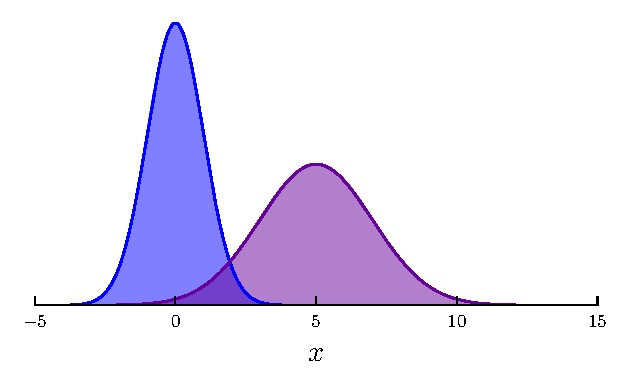
\includegraphics[width=.8\textwidth]{hist_normal.pdf}\\[-.8em]
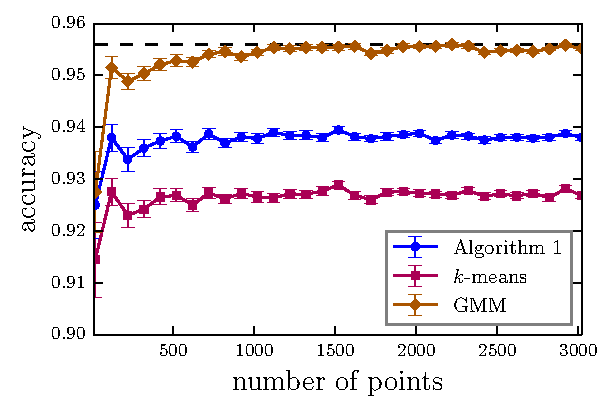
\includegraphics[width=\textwidth]{gauss1d.pdf}\\[-1em]
(a)
\end{minipage}
\begin{minipage}{0.49\textwidth}
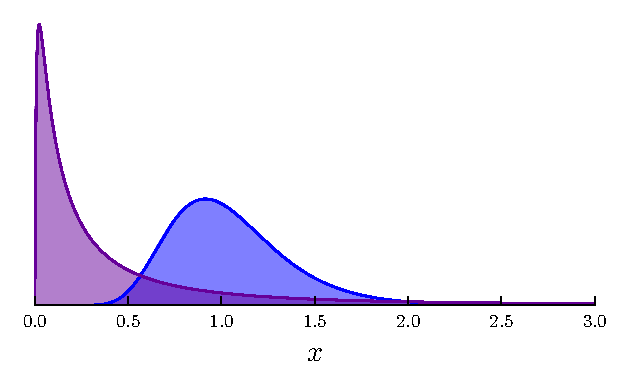
\includegraphics[width=.8\textwidth]{hist_lognormal.pdf}\\[-.8em]
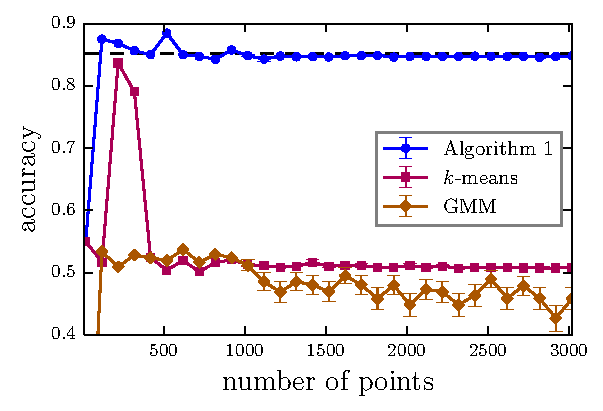
\includegraphics[width=\textwidth]{loggauss1d.pdf}\\[-1em]
(b)
\end{minipage}
\caption{
\label{fig:1d}
Energy statistics clustering by Algorithm~\ref{algo1d}
compared to $k$-means and GMM/EM.
We have the same number of points in both clusters, and for each case
we sample $100$ times from the distributions shown in the histograms. We 
plot the average value of 
\eqref{eq:accuracy} versus the total number of points 
(error bars are standard error). The dashed line indicates the
best possible classification accuracy computed from Bayes error.
(a) Data coming from \eqref{eq:two_normal}, where the
optimal accuracy is $\approx 0.956$.
(b) Data from \eqref{eq:two_lognormal}, where the optimal
accuracy is $\approx 0.852$.
}
\end{figure}

We now consider two simple experiments with equal number of points
in each cluster. We plot the accuracy \eqref{eq:accuracy} versus the number
of points in each cluster.
The data is clustered using 
the $\mathcal{E}^{1D}$-clustering algorithm,
% @gui: i see why you call this algorithm 1, but can we call it something with semantic meaning? like 1D-\mathcal{E}-clustering? or maybe \mathcal{E}1 for short? same for the other variants.
% @jovo: will call energy clustering, or $\mathcal{E}-clustering$ is name is to
% big when I regenerate the plots with new figures
GMM through EM algorithm, and $k$-means++ 
algorithm. 
% @gui: there are many k-means algorithms, be specific.
% @jovo: there is only one k-means no? Anything else I would call kernel
% k-means. I called $k$-means++ though
We use the initialization procedure from 
$k$-means++ \cite{Vassilvitskii} also for GMM.
We run the algorithms $10$
times choosing the result with  best objective function value. 
% @gui: a few? be specific
% @jovo: ok
Notice that $\mathcal{E}^{1D}$-clustering does not require any random
initialization so we only
% @gui: "no initiazation" is weird.  do any algs require an initialization?
% @jovo: I guess so. In this algorithm we just compute something "exactly",
% contrary to random initializing and iterating to optimize the solution.
% There is no random initialization in this algo
run it once.
Moreover, for each case we sample $100$ times
and show the average accuracy with error bars indicating
the standard error.
In  Fig.~\ref{fig:1d}a 
we have data sampled from two normal distributions with equal number of
points in each cluster,
\begin{equation}
\label{eq:two_normal}
x \sim \mathcal{N}\big(\mu_i,\sigma_i^2\big) 
\quad 
\mbox{with $\mu_1 = 0$, $\sigma_1=1$ and
$\mu_2 = 5$, $\sigma_2 = 2$.}
\end{equation}
For these distributions the optimal accuracy 
obtained from Bayes classification error
is $ \approx 0.956$ which is indicated by the dashed line in the plot.
We see that the three methods
perform closely. As expected, GMM has a slight advantage over the other
methods since
it corresponds to the true model of the data. 
Energy statistics performs slightly better
than $k$-means. On the other hand, in Fig.~\ref{fig:1d}b
we consider two clusters with lognormal distributions,
\begin{equation}
\label{eq:two_lognormal}
\log x \sim \mathcal{N}\big( \mu_i,\sigma_i^2\big) \quad
\mbox{with
$\mu_1 = 0$,
$\sigma_1 = 0.3$ and
$\mu_2 = -1.5$,
$\sigma_2 = 1.5$.}
\end{equation}
% @gui: why not use the same parameters as in fig 1a?  i feel like if we did, it would seem less like we are cherry picking?  
% @jovo: yes, and GMM would do great! In 1D is very hard to find setting where
% GMM and k-means perform poorly, so we have to cherry pick. In 1D you
% basically do not have much choice, if data has minimal separation k-means and
% GMM does well.
% The purpose is to
% illustrate that there are settings where k-means/GMM do poorly and energy
% does not. If I choose the same parameters as before all algorithms are doing
% great, sometimes GMM can even do better than energy.
The optimal classification accuracy from Bayes error is $\approx 0.852$.
% @gui: computed numerically?
% @jovo: yes!
In this case,
Algorithm~\ref{algo1d} provides a very accurate clustering while
GMM and $k$-means basically cluster at chance.
Sometimes GMM/EM  was unable to estimate the parameters 
thus giving zero accuracy.
The two simple experiments of Fig.~\ref{fig:1d} illustrate
how energy statistics clustering is nonparametric, being able
to provide high quality clustering in settings where data comes
from very different distributions.


%%%%%%%%%%%%%%%%%%%%%%%%%%%%%%%%%%%%%%%%%%%%%%%%%%%%%%%%%%%%%%%%%%%%%%%%%%%%%%%
\section{Iterative Algorithms for Energy Clustering}
\label{sec:algo}

In this section we introduce an iterative algorithm to find a local
maximizer of \eqref{eq:qcqp2}. Due to 
Proposition~\ref{th:kernel_kmeans} we can also find an approximate
solution by the well-known kernel $k$-means algorithm based
on Lloyd's heuristic (see \cite{Dhillon2,Dhillon}), which 
for convenience will also be restated in the present context.

Consider the optimization problem 
written in the form \eqref{eq:max_prob} as follows:
\begin{equation}
\label{eq:maxQ}
\max_{\{ \C_1,\dotsc,\C_k \}} 
\bigg\{ Q = \sum_{j=1}^k \dfrac{Q_j}{n_j}  \bigg\},
\qquad Q_j = \sum_{x,y\in\C_j} \kk(x,y),
\end{equation}
where $Q_j$ represents an internal energy cost of cluster $\C_j$, and
$Q$ is the total energy cost where each $Q_j$ 
is weighted by the inverse
of the number of its elements. For a data point $x_i$ we denote
its own energy cost
with the entire cluster $\C_\ell$ by
\begin{equation}
\label{eq:costxij}
Q_\ell(x_i) \equiv \sum_{y\in\C_\ell} \kk(x_i, y) = 
G_{i \bullet} \cdot Z_{\bullet \ell},
\end{equation}
where we recall that $G_{i\bullet}$ ($G_{\bullet i}$) denotes
the $i$th row (column) of matrix $G$.

%\subsection*{Kernel $\bm{k}$-Means Algorithm}
\subsection*{Lloyd's Method for Energy Clustering}

To optimize the kernel $k$-means objective function
\eqref{eq:J} we remove the global term and define the function
\begin{equation}
\label{eq:Jell}
J^{(\ell)}(x_i) \equiv 
\dfrac{1}{n_\ell^2} Q_\ell
-\dfrac{2}{n_\ell} Q_\ell(x_i) .
\end{equation}
We are thus solving 
\begin{equation}
\min_{Z} 
\sum_{i=1}^n 
\sum_{\ell=1}^k Z_{i\ell} J^{(\ell)}(x_i).
\end{equation}
One possible strategy is to
assign  $x_i$ to cluster $\C_{j^\star}$ according
to 
\begin{equation}
j^\star = \argmin_{\ell=1,\dotsc,k} J^{(\ell)}(x_i) .
\end{equation}
This is done for every data point $x_i$ and repeated until
convergence, i.e. until no new assignments are made.
The entire procedure is described in Algorithm~\ref{kmeans_algo}, which
we call $\mathcal{E}^L$-clustering to emphasize
that we are optimizing the energy function $W$ from energy statistics
based on Lloyd's method \cite{Lloyd}.
% @gui: let's call this something more informative
% @jovo: alright
It can be shown that this algorithm converges provided $G$ is positive
semidefinite. 

% @jovo: check this paragraph. I included it to answer your question
% about having K(x,x) and \ell=1,...,k without exluding \ell=j. Essentially,
% the term K(x,x) will be hidden inside the mean of the cluster to which
% x is currently assigned to. This also clarifies the connection to 
% the standard formulation of kernel k-means.
Actually, $\mathcal{E}^{L}$-clustering is preciselly
kernel $k$-means algorithm \cite{Dhillon2,Dhillon} 
but written in a more concise and clear manner. Indeed, recalling that
$\kk(x,y)=\langle \varphi(x), \varphi(y) \rangle$ where $\varphi: \mathcal{X}
\to \mathcal{H}_\kk$ is the feature map, we have from \eqref{eq:Jell} that
\begin{equation}
%\begin{split}
J^{(\ell)}(x_i) 
%&= \dfrac{1}{n_\ell^2} \sum_{x, y \in \C_\ell} 
%\langle \varphi(x), \varphi(y) \rangle - \dfrac{2}{n_\ell}
%\sum_{y\in \C_\ell} \langle \varphi(x_i), \varphi(y)\rangle \\ 
= 
\langle \varphi(\mu_\ell), \varphi(\mu_\ell) \rangle
-2 \langle \varphi(x_i), \varphi(\mu_\ell) \rangle 
= 
\| \varphi(x_i) - \varphi(\mu_\ell) \|^2 - \| \varphi(x_i) \|^2,
%\end{split}
\end{equation}
where $\mu_\ell = \tfrac{1}{n_\ell} \sum_{x\in \C_\ell}x$ 
is the mean (center) of cluster $\C_\ell$. 
Therefore, $\min_\ell J^{(\ell)}(x_i) = 
\min_\ell \| \varphi(x_i) - \varphi(\mu_\ell)\|^2$, i.e. we are assigning
$x_i$ to the cluster with closest center (in feature space),
which is the familiar Lloyd's
heuristic approach.

To check the complexity of $\mathcal{E}^L$-clustering, 
notice that to compute the second term of $J^{(\ell)}(x_i)$
in \eqref{eq:Jell} requires
$\OO(n_\ell)$ operations, and although the first term requires
$\OO(n_\ell^2)$ it only needs to be computed once outside loop through
data points (step 1 of Algorithm~\ref{kmeans_algo}).
Therefore, the time complexity of $\mathcal{E}^L$-clustering 
is
$\OO(n k \max_\ell n_\ell) = \OO(k n^2)$. For a sparse
Gram matrix $G$ having
$n'$ nonzero elements this complexity can be further reduced
to $\OO(k n')$. 

\begin{figure}
\begin{flushleft}
\begin{algorithm}[H]
\vspace{.5em}
\begin{algorithmic}[1]
    \INPUT number of clusters $k$, Gram matrix $G$, initial label
    matrix $Z \leftarrow Z_0$
    \OUTPUT label matrix $Z$ 
  \STATE $q \leftarrow (Q_1, \dotsc, Q_k)^\top$ 
            have the costs of each cluster, defined in \eqref{eq:maxQ}
  \STATE $n \leftarrow (n_1,\dotsc,n_k)^\top$ 
        have the number of points in each cluster%, obtained 
        %from $D = Z^\top Z$
  \REPEAT
    \FOR{ $i=1,\dotsc,n$}
        \STATE let $j$ be such that $x_i \in \C_j$
        \STATE $j^\star \leftarrow \argmin_{\ell=1,\dotsc,k} J^{(\ell)}(x_i)$,
            where $J^{(\ell)}(x_i)$ is defined in \eqref{eq:Jell}
            %, for $\ell=1,2,\dots,k$
        \IF{ $j^\star \ne j$} 
            \STATE move $x_i$ to $\C_{j^\star}$: $Z_{ij} \leftarrow 0$ and
            $Z_{ij^\star} \leftarrow 1$
            \STATE update $n$: $n_j \leftarrow n_j - 1$ and
                    $n_{j^\star} \leftarrow n_{j^\star} + 1$
            \STATE update $q$: $q_j \leftarrow q_j - 2Q_j(x_i)$ and
    $q_{j^\star} \leftarrow q_{j^\star} + 2Q_{j^\star}(x_i)$
    %    \ELSE
    %        \STATE Do nothing;
        \ENDIF
    \ENDFOR
  \UNTIL{convergence}
\end{algorithmic}
\caption{\label{kmeans_algo}
$\mathcal{E}^{L}$-clustering: Lloyd's method for energy clustering, which
is preciselly kernel $k$-means algorithm. This procedure finds
local solutions to the problem \eqref{eq:qcqp2}.
}
\end{algorithm}
\end{flushleft}
\end{figure}

\subsection*{Hartigan's Method for Energy Clustering}

We now consider Hartigan's method \cite{Hartigan} 
applied to the optimization problem in the form \eqref{eq:maxQ}, which gives
a local solution to the QCQP defined in \eqref{eq:qcqp2}. 
The method is based in computing the maximum change
in the total cost function $Q$ when moving each data point to
another cluster. More specifically, 
suppose point $x_i$
is currently assigned to  cluster $\C_j$ yielding
a total cost function denoted by $Q^{(j)}$.
Moving $x_i$ to cluster $\C_\ell$ yields another total cost function
denoted by $Q^{(\ell)}$. We are interested in computing the maximum 
cost change
$\Delta Q^{j\to \ell} (x_i) \equiv Q^{(\ell)} - Q^{(j)}$, for $\ell\ne j$. 
From \eqref{eq:maxQ}, by explicitly writting the costs related to these 
two cluster we obtain
\begin{equation}
\Delta Q^{j\to \ell} (x_i) = \dfrac{Q_\ell^{+}}{n_\ell+1} + 
\dfrac{Q_j^-}{n_j-1} - \dfrac{Q_j}{n_j} - \dfrac{Q_\ell}{n_\ell}
\end{equation}
where $Q^{+}_\ell$ denote the cost of the new $\ell$th cluster
with the point $x_i$ added to it, and $Q^-_j$ is the cost of new 
$j$th cluster with $x_i$ removed from it. Noting that 
$Q_\ell^{+} = Q_\ell + 2 Q_\ell(x_i) + G_{ii}$ and
$Q_j^{-} = Q_j - 2 Q_j(x_i) + G_{ii}$, we get the formula
\begin{equation}
\label{eq:changeQ}
\Delta Q^{j \to \ell}(x_i)  = 
\dfrac{1}{n_j - 1}\left[ \dfrac{Q_j}{n_j} - 2 Q_j(x_i) + G_{ii} \right]
- \dfrac{1}{n_\ell + 1}\left[ \dfrac{Q_\ell}{n_\ell} - 2 Q_\ell(x_i) 
- G_{ii} \right].
\end{equation}
Therefore, if $\Delta Q^{j\to \ell}(x_i) > 0$ we get closer to a 
maximum of \eqref{eq:maxQ} by
moving $x_i$ to $\C_\ell$, otherwise we keep $x_i$ in $\C_j$. Based on
this the proposed algorithm goes as follows.
We start with an initial configuration for the label matrix $Z$, 
then for each
point $x_i$ 
we compute the cost of moving it to another cluster $\C_\ell$, i.e.
$\Delta Q^{j\to \ell}(x_i)$ for 
$\ell=1,\dots,k$ with $\ell \ne j$ and $j$ denotes the index of its current
partition, $x \in \C_j$. Hence, we choose
\begin{equation}
j^\star = \argmax_{\ell=1,\dotsc,k \, | \, \ell\ne j} 
\Delta^{j \to \ell}(x_i).
\end{equation}
If $\Delta Q^{j \to j^\star}(x_i) > 0$ 
we move $x_i$ to cluster $\C_{j^\star}$, otherwise 
we keep $x_i$ in its original cluster $\C_j$. 
This process is repeated
until no points are assigned to new clusters. 
The entire procedure is explicitly described in Algorithm~\ref{algo}, which we
coin $\mathcal{E}^H$-clustering to emphasize that it is based on
Hartigan's method.
This method automatically ensures that the objective function is
monotonically increasing at each iteration, and consequently the algorithm
converges in a finite number of steps.

\begin{figure}
\begin{flushleft}
\begin{algorithm}[H]
\vspace{.5em}
\begin{algorithmic}[1]
    \INPUT number of clusters $k$, Gram matrix $G$, 
                initial label matrix $Z \leftarrow Z_0$
    \OUTPUT label matrix $Z$
  \STATE $q \leftarrow (Q_1, \dotsc, Q_k)^\top$ 
            have the energy costs of each cluster, defined in \eqref{eq:maxQ}
  \STATE $n \leftarrow (n_1,\dotsc,n_k)^\top$ have the number of points 
        in each cluster%, obtained from $D=Z^\top Z$
  \REPEAT
    \FOR{ $i=1,\dotsc,n$}
        \STATE let $j$ be such that $x_i \in \C_j$
        \STATE $j^\star \leftarrow \argmax_{\ell=1,\dotsc,k \, | \, \ell\ne j} 
                \Delta Q^{j\to \ell}(x_i)$
            %for $\ell=1,2,\dots,k$ and $\ell \ne j$; 
            using Eq. \eqref{eq:changeQ} \label{stepmove}
        \IF{ $\Delta Q^{j \to j^\star}(x_i) > 0$ }
            \STATE move $x_i$ to $\C_{j^\star}$: $Z_{ij} \leftarrow 0$ and 
            $Z_{ij^\star} \leftarrow 1$
            \STATE update $n$: $n_j \leftarrow n_j - 1$ and
                    $n_{j^\star} \leftarrow n_{j^\star} + 1$
            \STATE update $q$: $q_j \leftarrow q_j - 2Q_j(x_i) + G_{ii}$ and
    $q_{j^\star} \leftarrow q_{j^\star} + 2Q_{j^\star}(x_i)+ G_{ii}$
    %    \ELSE
    %        \STATE Do nothing;
        \ENDIF
    \ENDFOR
  \UNTIL{convergence}
\end{algorithmic}
\caption{\label{algo}
$\mathcal{E}^H$-clustering: Hartigan's method for energy clustering.
This algorithm finds local solutions to  
the optimization problem \eqref{eq:qcqp2}.
\hspace{\fill}
}
\end{algorithm}
\end{flushleft}
\end{figure}

The complexity analysis of $\mathcal{E}^H$-clustering is the following.
Computing the Gram matrix $G$ requires $\OO( D n^2)$ operations, where 
$D$ is the dimension of each data point and $n$ is the data size. However,
both algorithms $\mathcal{E}^L$- and $\mathcal{E}^H$-clustering 
assume that $G$ is given. There are more efficient
methods to compute $G$, specially if it is sparse, but we will not consider
this further and just assume that $G$ is given.
The computation of each cluster cost
$Q_j$ has complexity $\OO(n_j^2)$, and overall to compute $q$
we have $\OO(n_1^2+\dots + n_k^2) = \OO(k \max_j n_j^2)$. 
These operations only need to be performed a single time. For
each point $x_i$ we need to compute $Q_j(x_i)$ once, which is
$\OO(n_j)$, and we need to compute $Q_\ell(x_i)$ for each $\ell\ne j$. 
The cost of computing 
\eqref{eq:costxij} is $\OO(n_j)$, thus the cost of step~$8$ in
Algorithm~\ref{algo} is $\OO(k \max_j n_j)$ for $j=1,\dotsc,k$.
For the 
entire dataset this gives a time complexity
of $\OO(n k  \max_j n_j) =\OO(k n^2)$. Note that this is the same cost as
in $\mathcal{E}^L$-clustering, or kernel $k$-means algorithm. 
Again, if $G$ is sparse
this can be reduced to $\OO(k n')$ where $n'$ is the number of nonzero
entries of $G$.

In the following we mention some important known 
results about Hartigan's method.
% @gui: "let us" again...
% @jovo: ok

\begin{theorem}[Telgarsky-Vattani \cite{Telgarsky}]
Hartigan's method has the cost function strictly decreasing in each
iteration. Moreover, if $n > k$ then 
\begin{enumerate}
\item \label{noempty} the resulting partition has no empty clusters, and
\item \label{diffmean} the resulting partition has distinct means.
\end{enumerate}
\end{theorem}

%Both conditions of the  above theorem are not satisfied 
%by Lloyd's method, 
Neither of these two conditions are guaranteed to be 
satisfied  by Lloyd's method,
% @gui: do you mean Lloyd's method satisfies neither, or does not satisfy both?  please clarify
% @jovo: ok
and consequently by $\mathcal{E}^L$-clustering 
algorithm.
The next result indicates that Hartigan's method can potentially 
escape local optima of Lloyd's method.

\begin{theorem}[Telgarsky-Vattani \cite{Telgarsky}]
The set of local optima of Hartigan's method is a (possibly strict) subset
of local optima of Lloyd's method.
\end{theorem}

The above theorem implies that $\mathcal{E}^L$-clustering  cannot
improve on a local optima of $\mathcal{E}^H$-clustering. On the other hand,
$\mathcal{E}^H$-clustering might improve on a local optima of 
$\mathcal{E}^L$-clustering. Lloyd's method forms Voronoi partitions,
while Hartigan's method groups data
in regions formed by the intersection of spheres called circlonoi cells.
It can be shown that the circlonoi cells are contained within
a smaller volume of a Voronoi cell, and this excess volume grows
exponentially with the dimension of $\mathcal{X}$ 
\cite[Theorems 2.4 and 3.1]{Telgarsky}. 
Points in this excess volume
force Hartigan's method to iterate, contrary
to Lloyd's method. Therefore, Hartigan's 
can escape local
optima of Lloyd's. 
Moreover, this improvement should be more prominent as
dimension increases. Also, the improvement grows as $k$
increases.
The empirical results of \cite{Telgarsky} show that 
an implementation of Hartigan's method has comparable execution time 
as an implementation of
Lloyd's method,
but no explicit complexity was provided. In our case, we showed that both
$\mathcal{E}^L$- and $\mathcal{E}^H$-clustering
have the same time complexity. 

In \cite{Slonin} Hartigan's method was applied to $k$-means problem
with any Bregman divergence. It was shown that the number of Hartigan's
local minima is upper bounded by $\mathcal{O}(1/k)$ 
\cite[Proposition 5.1]{Slonin}. 
In addition, it was provided examples where
\emph{any} initial partition correspond to a local optima of Lloyd's 
method, while  the number of local optima in Hartigan's method is small and 
correspond to true partitions of the data. Empirically, the number of
Hartigan's local optima was considerably smaller than the number of Lloyd's
local optima.

The above results indicate that Hartigan's method
provides several advantages over Lloyd's method, a fact that will also
be supported by our numerical experiments in the next section where 
$\mathcal{E}^H$-clustering  outperforms
of $\mathcal{E}^L$-clustering (kernel $k$-means) in several settings.


%%%%%%%%%%%%%%%%%%%%%%%%%%%%%%%%%%%%%%%%%%%%%%%%%%%%%%%%%%%%%%%%%%%%%%%%%%%%%%%
\section{Numerical Experiments}
\label{sec:numerics}

In the experiments below we fix the semimetric 
according to the traditional energy distance \eqref{eq:energy}, and
the point $x_0=0$ is chosen in the corresponding kernel  
\eqref{eq:kernel_semimetric}. We therefore use
\begin{equation}
\label{eq:standard_metric}
\rho(x,y) = \| x-y\| \qquad \mbox{and} \qquad \kk(x,y) = 
\tfrac{1}{2}\left( \| x \| + \| y \| - \| x-y \| \right).
\end{equation}
We will consider other kernels as well 
but \eqref{eq:standard_metric} will be the
standard kernel for energy statistics and will always be present in the
experiments as a reference.

Let us briefly mention that we compared $\mathcal{E}^H$-clustering,
as described in Algorithm~\ref{algo}, to
the $1D\,\mathcal{E}$-clutering, described in Algorithm~\ref{algo1d}, 
for several univariate distributions.
Both perform almost indistinguishable regarding the clustering quality.
However, we omit these results since we will analyse more interesting 
scenarios in high dimensions and $k > 2$ number of clusters.

The main goal of the 
experiments  to follow
is to compare Algorithm~\ref{algo} based on Hartigan's method to
kernel $k$-means, as described in Algorithm~\ref{kmeans_algo}, which
is based on Lloyd's method. 
% @gui: i might call them \mathcal{E}-H & \mathcal{E}-L, or some such?
% @jovo: it might be a good idea, let's decide when I re-do the plots
From the discussion in the end of the previous section we can anticipate
that Algorithm~\ref{algo} will be superior than Algorithm~\ref{kmeans_algo}.
Another goal is to illustrate the nonparametric aspect of energy statistics.
To this end we also compare
Algorithm~\ref{algo} to standard $k$-means and GMM/EM since 
these are reference
clustering algorithms in practice.
Moreover, for every algorithm, we always
choose the initialization procedure from $k$-means++%
\footnote{Notice that we just use the initialization
procedure and not the full $k$-means++ algorithm.} \cite{Vassilvitskii}.
Our measure of clustering quality will be the accuracy \eqref{eq:accuracy}
based on the ground truth. Furthermore, in every experiment, we sample
data many times and show the average value of the accuracy with error bars
indicating the standard error. Whenever possible, 
% @gui: bayes error is always possible to numerically estimate, no? maybe sometimes computationally intractable?
% @jovo: true. I just didn't indicate Bayes error for Fig. 3 for instance cuz
% will be very boring, will have to compute for every number of points, and
% also we don't do that for MNIST and circles, thus the phrase
we also indicate the optimal 
accuracy computed from
Bayes classification error.

From the results of \cite{Telgarsky}, we expect the improvement of Hartigan's 
over Lloyd's method to be more accentuated in high dimensions.
Thus, we analyze
how the algorithms degrade as the number of dimensions increase, while
keeping the number of points in each cluster fixed. Consider
two clusters with multivariate normal distributions given by
\begin{equation}
\label{eq:gauss1}
\begin{split}
x &\in \C_i  \sim 
\mathcal{N}(\mu_i,\Sigma_i) \qquad (i=1,2),  \\
\mu_1 &= (\underbrace{0,\dotsc,0}_{\times D})^\top , \quad
\mu_2 = 0.7 \times (\underbrace{1,\dots,1}_{\times 10},
\underbrace{0,\dots,0}_{\times (D-10)})^\top, \quad
\Sigma_1 = \Sigma_2 = I_D.
\end{split}
\end{equation}
Note that the Bayes error
is fixed as $D$ increases, giving an optimal 
accuracy of $\approx 0.86$.
For each $D$ we generate $100$ Monte Carlo runs, 
sampling $100$ points for each cluster.
% @gui: if you sample 100 points from each cluster, it breaks the GMM model, which assumes you sample n_i points from cluster i with probability \pi_i.  i don't think it matters that much, but good to know :)
% @jovo: humm ... true, didn't think about that. Do you think I should re-do
% all experiments in this way? sampling from clusters with prob 1/2 for
% instance, instead of exactly picking a fixed number of points for each?
We apply each algorithm to the resulting dataset 
and compute the average of the accuracy \eqref{eq:accuracy} (error bars
are standard error).
Algorithm~\ref{algo} and Algorithm~\ref{kmeans_algo} 
both use the standard
kernel \eqref{eq:standard_metric}.
The results are shown in Fig.~\ref{fig:gauss}a.
Note that GMM/EM is unable to estimate the covariance matrices
when the number of dimensions exceeds the number of points in each cluster,
%giving zero accuracy when dimensions are $\gtrsim 100$.
i.e. when $D \gtrsim 100$.
We see that Algorithm~\ref{algo} performs better than all the other ones,
and in particular it outperforms kernel $k$-means, Algorithm~\ref{kmeans_algo},
as the number
of dimensions increase. 
% @gui: when you say "kernel k-means" here, do you mean algorithm 2?  if so, please clarify, if not, please clarify :)
% @jovo: will change again when we introduce algorithm's names

%Note also that although GMM and $k$-means are
%parametric they are consistent models to the data.
Note that in this case GMM and $k$-means are consistent estimators.

% @gui: gmm & k-means are not 'models". they are algorithms, or in this context, they are estimators.
% @jovo: see if it's correct now. 
% Don't know how to say this, what I wanted to say is
% that GMM and k-means are algorithms that were built based on gaussian
% mixtures models, and they should perform close to optimal when data
% is normally distributed.

\begin{figure}
\begin{minipage}{0.49\textwidth}
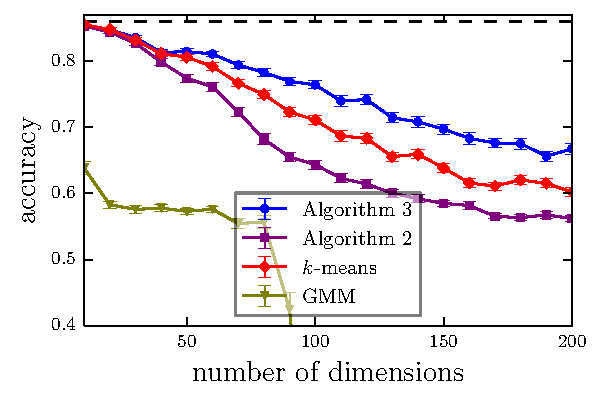
\includegraphics[width=1\textwidth]{gauss_dim.pdf}\\[-1.0em] (a)
\end{minipage}
\begin{minipage}{0.49\textwidth}
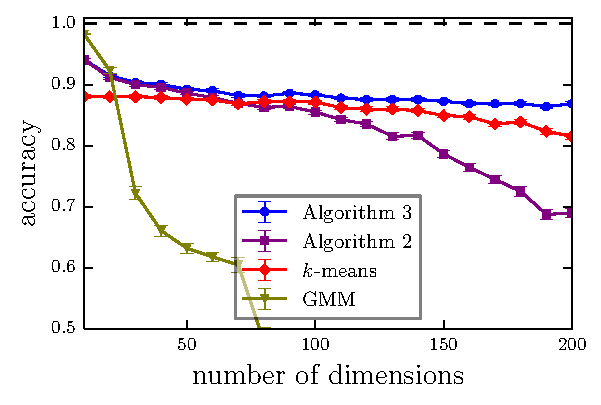
\includegraphics[width=1\textwidth]{gauss_cov_squareroot.pdf}\\[-1.0em] (b)
\end{minipage}
\begin{minipage}{0.49\textwidth}
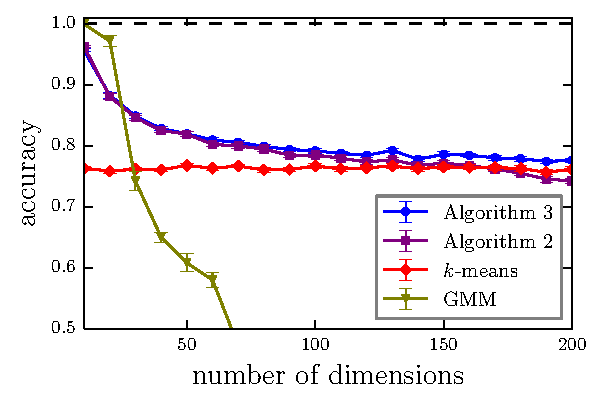
\includegraphics[width=1\textwidth]{gauss_cov_linear.pdf}\\[-1.0em] (c)
\end{minipage}
\begin{minipage}{0.49\textwidth}
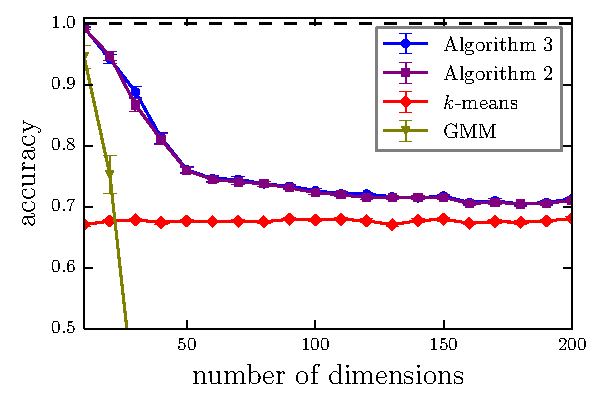
\includegraphics[width=1\textwidth]{gauss_cov_square.pdf}\\[-1.0em] (d)
\end{minipage}
\caption{
\label{fig:gauss}
Comparison of Algorithm~\ref{algo}, Algorithm~\ref{kmeans_algo},
standard $k$-means and GMM/EM as the number of dimensions increase
in Gaussian settings.
% @gui: gaussian is always captilized
% @gui: also, i don't understand this plot entirely, are you really starting with D=1? or 10? from the equations, it would seem that Bayes error changes when D< 10, but your Bayes error lines do not seem to change?
% @jovo: I start with D = 10.
% @gui: cep points out that in Fig 2a, GMM does very poorly even with d small, which does not make sense to us.  can you explain?
% @jovo: you're right, didn't realize that. Will double check and maybe repeat
% the experiment.
We compute the average of \eqref{eq:accuracy} over $100$ samples with
error bars being standard error. We have two clusters with $100$ points
each. 
(a) Data as in \eqref{eq:gauss1}, where the optimal accuracy
from Bayes error is the dashed line equal to $\approx 0.86$.
(b) Data from \eqref{eq:gauss2} with $q=1/2$ in \eqref{eq:cov}. 
(c) Data from \eqref{eq:gauss2} with $q=1$ in \eqref{eq:cov}.
(d) Data from \eqref{eq:gauss2} with $q=2$ in \eqref{eq:cov}.
The optimal accuracy from Bayes error in (b--d) is $\approx 1$.
% @gui: titles for each, or subcaptions, would be extremely useful.  in general, titles should provide the "setting" of the experiment, ie, the model, etc.
% @jovo: ok will do when I re-generate the plots.
% @gui: also helpful here would be pairs plots, say, of the first 5 dimensions, showing the performance of our stuff (color points by Alg 3, maybe symbols denote "truth".  i have no intuition how difficult these are.
% @jovo: didn't understand this
}
\end{figure}

%Let us now consider the same experiment as before with data distributed as
Consider now the following setting:
% @gui: what do you mean "the same experiment as before"? clarify, or don't say that. there are obviously differences. 
% @jovo: ok
\begin{equation}
\label{eq:gauss2}
x \in \C_i  \sim 
\mathcal{N}(\mu_i,\Sigma_i) \quad (i=1,2),  \quad
\mu_1 = (\underbrace{0,\dotsc,0}_{\times D})^\top , \quad
\mu_2 = (\underbrace{1,\dots,1}_{\times 10},
\underbrace{0,\dots,0}_{\times (D-10)})^\top, 
\end{equation}
where
\begin{equation}
\label{eq:cov}
(\Sigma_1)_{ij} = \begin{cases}
i^{-q} \delta_{ij} & \mbox{if $i \le 10$} \\
\delta_{ij} & \mbox{if $10 < i \le D$}
\end{cases} \qquad
(\Sigma_2)_{ij} = \begin{cases}
i^{\,q} \delta_{ij} & \mbox{if $i \le 10$} \\
\delta_{ij} & \mbox{if $10 < i \le D$}
\end{cases} 
\end{equation}
and we choose $q \in \{ 1/2, 1, 2\}$. Above $\delta_{ij} = 1$ if $i=j$ and
$\delta_{ij}=0$ if $i\ne j$ is the Kronecker delta. In these cases,
% @gui: what is delta_ij??? can you explain the intuition for this setting, i don't get it, maybe because i don't know what delta_ij is.....
% @jovo: delta_{ij} is the Kronecker delta, I included the definition
the best possible accuracy from Bayes classification error is $\approx 1$.
In Fig.~\ref{fig:gauss}b--d we have $q=1/2$, $q=1$, and $q=2$, respectivelly.
Again, GMM/EM is unable to estimate the covariance matrices
as dimensions get larger than $\gtrsim 100$, and it gives poor results even
for number of dimensions much lower than this. Note that GMM requires
a larger number of points to estimate the parameters accurately.
Algorithm~\ref{algo} outperforms
Algorithm~\ref{kmeans_algo}, and $k$-means degrades faster as 
$q$ increases.

To summarize, in the experiments of Fig.~\ref{fig:gauss}
we see a better performance of Algorithm~\ref{algo} compared
to the other ones, and in particular to kernel $k$-means,
where we recall that both find local solutions
to the same optimization problem \eqref{eq:qcqp2}.
Algorithm~\ref{algo} is more robust as the number of dimensions
increase.
% @gui: is there any reason to initialize alg 3 with alg 2? is it even worth trying?
% @jovo: based on the theorems I cited for Hartigan's this is actually worse,
% since the set of local minima of Hartigan's is a subset of Lloyd's, thus if
% you do that Hartigan's may not iterate. However, Hartigan's has possibly less
% local minima than Lloyd's so if you start at random, or not on a local
% minima it may converge to a better solution

Consider the effect of having 
unbalanced clusters according to
\begin{equation}
\label{eq:gauss3}
\begin{split}
x &\in \C_i \sim  
\dfrac{n_i}{N} \mathcal{N}(\mu_i,\Sigma_i) \quad (i=1,2), \quad 
\mu_1 = (0,0,0,0)^\top , \quad
\mu_2 = 1.5\times (1,1,0,0)^\top, \\
\Sigma_1 &= I_4, \quad
\Sigma_2 = \left( 
\begin{smallmatrix} 
1/2 & 0 & 0 & 0\\
0 & 1/2 & 0 & 0 \\
0 & 0 & 1 & 0 \\
0 & 0 & 0 & 1 
\end{smallmatrix}\right), \quad
n_1 = N - m, \quad  n_2 = N + m, \quad N=200.
\end{split}
\end{equation}
We then increase $m$, 
that is we make the clusters progressively more unbalanced,
and plot the average of \eqref{eq:accuracy} 
over
$100$ samples for each $m$
(error bars are standard error). The results are in Fig.~\ref{fig:unbalanced}.
For highly unbalanced clusters we see that GMM performs better than
the other methods which have similar performance.
%As expected, GMM
%works better than the other algorithms since it is a fuzzy clustering.
%The other methods based on hard assignments degrade similarly
%and  more rapidly than GMM. This indicates that a soft version of
%Algorithm~\ref{algo} should compensate for this effect.
% @gui: in stats, we don't say "fuzzy", we say "soft".  also, why do you think that when clusters are imbalanced that soft clustering is more important? i would say that soft clustering is more important when the cluster centers are close, i don't see how imbalanced matters.
% @jovo: you are probably right, I'll remove this phrase. 
% I thought that this should be the case because in this setting that's pretty
% much the only difference between GMM and k-means

\begin{figure}
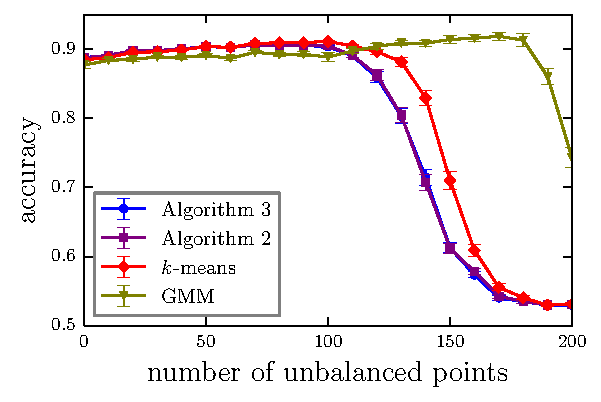
\includegraphics[width=0.5\textwidth]{gauss_pi.pdf}\vspace{-1em}
\caption{
\label{fig:unbalanced}
Comparison of Algorithm~\ref{algo}, Algorithm~\ref{kmeans_algo}, 
$k$-means, and GMM/EM. The data is distributed as \eqref{eq:gauss3} where
we make the clusters progressively more unbalanced.
}
\end{figure}

Besides the standard kernel from energy statistics 
\eqref{eq:standard_metric} 
% @gui: please remove all "let us" from manuscript
% @jovo: ok, hunting them
consider the following two other semimetrics with their respective generating
kernels:
\begin{align}
\rho_{1/2}(x,y) &= \| x-y \|^{1/2} & 
 \kk_{1/2}(x,y) &= \tfrac{1}{2} \left( 
\| x \|^{1/2} + \| y \|^{1/2} 
- \| x-y \|^{1/2} \right), \label{eq:rhohalf}\\
\rho_{e}(x,y) &= 
2 - 2 e^{-\tfrac{1}{2}\| x- y\|} &
 \kk_{e}(x,y) &= e^{-\tfrac{1}{2}\| x-y\|}.
\label{eq:rhoe}
\end{align}
The kernel $K_{1/2}(x,y)$ corresponds to the energy distance
\eqref{eq:energy2} with $\alpha=1/2$.
We sample data from the following normal distribution in $D=20$:
\begin{equation}
\label{eq:20gauss}
\begin{split}
x &\in \C_i \sim \mathcal{N}(\mu_i,\Sigma_i) \qquad (i=1,2), \\
\mu_1 &= (\underbrace{0,\dotsc,0}_{\times 20})^\top ,\quad
\mu_2 = \tfrac{1}{2} 
(\underbrace{1,\dotsc,1}_{5},\underbrace{0,\dotsc,0}_{15})^\top, \quad
\Sigma_1 = \tfrac{1}{2} I_{20},  \quad
\Sigma_2 = I_{20}.
\end{split}
\end{equation}
We sample an equal number of points for each cluster, which is progressively
increased. The optimal accuracy based on Bayes
classification error is $\approx 0.90$. 
Clustering results are shown in Fig.~\ref{fig:consist}a.
Algorithm~\ref{algo} outperforms the other ones, and in 
particular the kernel \eqref{eq:rhoe} provides better results.
As the number of points get large enough GMM starts to approach
optimal Bayes, as it should since it is a
consistent model to the data. However, 
Algorithm~\ref{algo} with kernel \eqref{eq:rhoe} approach optimal Bayes
with a much smaller number of points. Moreover, Algorithm~\ref{algo} 
outperforms
Algorithm~\ref{kmeans_algo} for any of the kernel choices.
% @gui: this is a separate point, that i would make a separate figure for if you want to make it. then, one fig would show E-H with 3 kernels vs. kmeans & gmm, and then another would show the difference between accuracy of E-H vs E-L for each of the 3 kernels.
% @jovo: ok, point taken, will come together with other plots

Now consider the same parameters as in \eqref{eq:20gauss} but with
lognormal distributions, 
\begin{equation}
\label{eq:20loggauss}
\log x \in \C_i \sim \mathcal{N}(\mu_i, \Sigma_i) \qquad (i=1,2).
\end{equation}
The same previous experiment is shown in 
Fig.~\ref{fig:consist}b.
Note that Algorithm~\ref{algo} still performs accurately, 
while $k$-means works almost at chance,
and GMM is not even able to estimate the parameters. 
% @gui: something is weird with the way you care computing accuracy.  GMM should not be significantly worse than chance.  i think you are probably counting the NaN's as *wrong*, rather than nothing?
% @jovo: yes, double checking that
Again, the
kernel \eqref{eq:rhoe}
provides better results than \eqref{eq:standard_metric} or
\eqref{eq:rhohalf}. 
The experiments in Fig.~\ref{fig:consist}
illustrate how energy statistics clustering is nonparametric.

\begin{figure}
\begin{minipage}{0.49\textwidth}
\centering
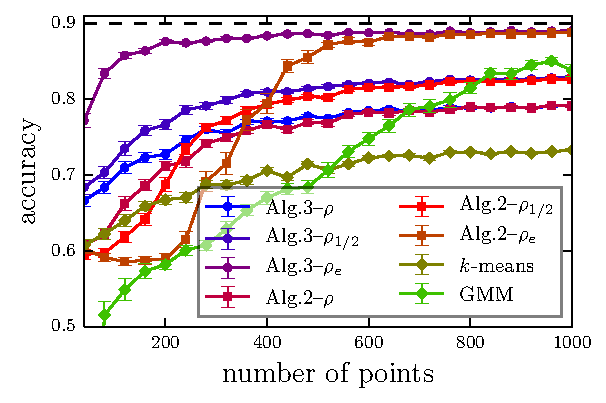
\includegraphics[width=1\textwidth]{gauss.pdf}\\[-1.0em]
(a)
\end{minipage}
\begin{minipage}{0.49\textwidth}
\centering
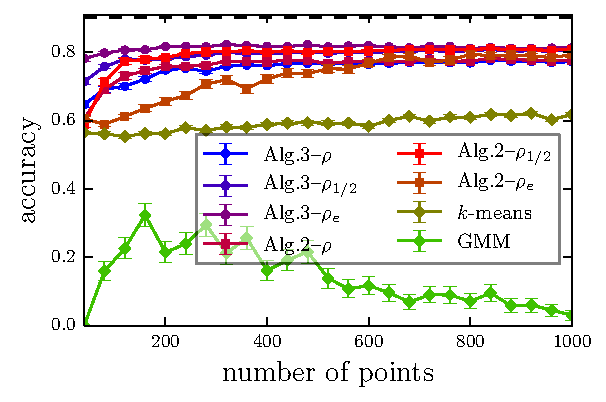
\includegraphics[width=1\textwidth]{loggauss.pdf}\\[-1.0em]
(b)
\end{minipage}
\caption{
\label{fig:consist}
% @gui: too many lines, you demonstrated that E-H is better than E-L already, i don't think we need to show the E-L variants here.
% @jovo: will fix that
Algorithm~\ref{algo} and Algorithm~\ref{kmeans_algo} with kernels
\eqref{eq:standard_metric}, \eqref{eq:rhohalf} and \eqref{eq:rhoe}, 
$k$-means, and GMM. The optimal accuracy in both cases
is $\approx 0.9$. We show the average of \eqref{eq:accuracy}
over $100$ samples with standard error.
(a) Data distributed as in 
\eqref{eq:20gauss}. 
(b) Data distributed as in \eqref{eq:20loggauss}.
}
\end{figure}


\begin{figure}
\begin{minipage}{0.24\textwidth}
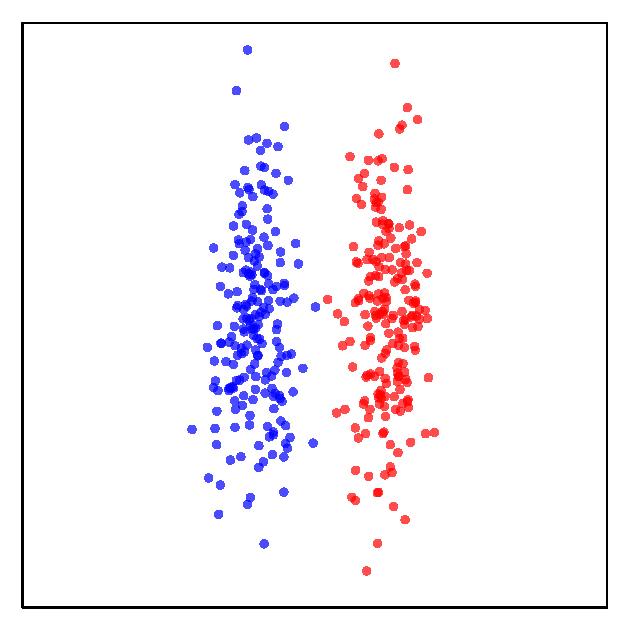
\includegraphics[width=1\textwidth]{2cigars.pdf}\\[-1em] (a)
\end{minipage}
\begin{minipage}{0.24\textwidth}
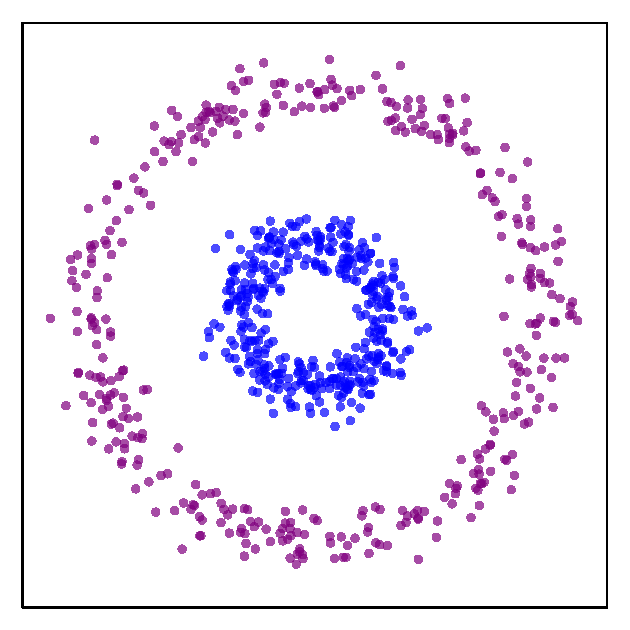
\includegraphics[width=1\textwidth]{2circles.pdf}\\[-1em] (b)
\end{minipage}
\begin{minipage}{0.24\textwidth}
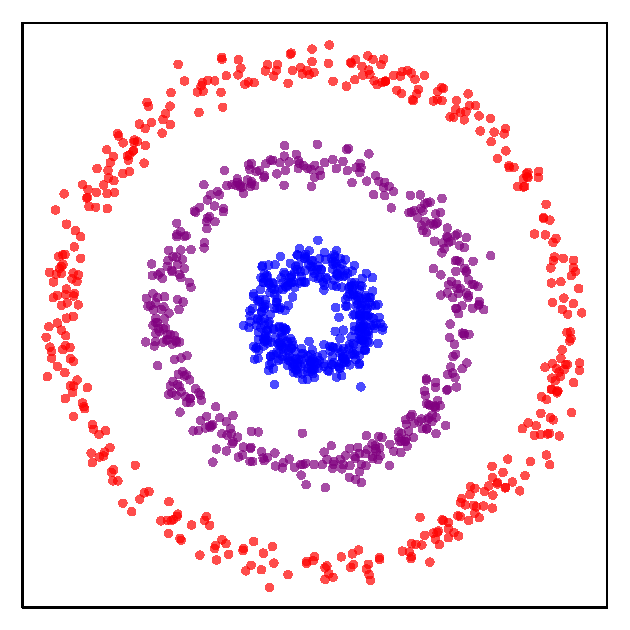
\includegraphics[width=1\textwidth]{3circles.pdf}\\[-1em] (c)  
\end{minipage}
\begin{minipage}{0.23\textwidth}
\vspace{-0.9em}
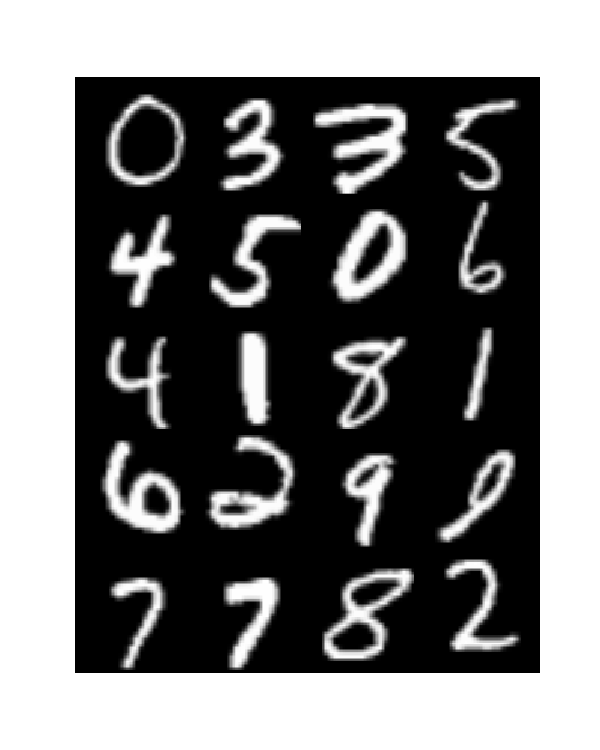
\includegraphics[width=1\textwidth]{mnist.pdf}\\[-1.8em] (d)  
\end{minipage}
\caption{\label{fig:other}
(a) Parallel cigars. (b) Two  
concentric circles with noise. (c) Three
concentric circles with noise. (d) MNIST handwritten digits.
Clustering results are in Table~\ref{table:other}
and Table~\ref{table:mnist}.
}
\end{figure}

Consider the following choices of semimetric and 
corresponding generating kernel:
\begin{align}
\rho_{\alpha}(x,y) &= \| x - y\|^\alpha & 
\kk_{\alpha}(x,y) &= \tfrac{1}{2}\left(
\| x \|^\alpha +
\| y \|^\alpha -
\| x-y \|^\alpha \right) ,
\label{eq:rhoalpha} \\
%
\widetilde{\rho}_{\sigma}(x,y) &= 2 - 2 e^{-\tfrac{\|x-y\|}{2 \sigma}} &
\widetilde{\kk}_{\sigma}(x,y) &= e^{-\tfrac{\|x-y\|}{2\sigma}} ,
\label{eq:rhoesigma} \\
%
\widehat{\rho}_{\sigma}(x,y) &= 2 - 2 e^{-\tfrac{\|x-y\|^2}{2 \sigma^2}} &
\widehat{\kk}_{\sigma}(x,y) &= e^{-\tfrac{\|x-y\|^2}{2\sigma^2}} .
\label{eq:rhogsigma} 
\end{align}
In Fig.~\ref{fig:other} we have examples of
complex two dimensional datasets. The two parallel cigars of 
Fig.~\ref{fig:other}a have $200$ points each. For the concentric circles
of Fig.~\ref{fig:other}b and Fig.~\ref{fig:other}c we
sample $400$ points for each class.
We apply Algorithm~\ref{algo} and Algorithm~\ref{kmeans_algo}, 
using the above kernels 
\eqref{eq:rhoalpha}--\eqref{eq:rhogsigma}, as well as
$k$-means and GMM. The results are shown
in Table~\ref{table:other} where the respective choice of parameters for the
kernels are indicated. For the data in Fig.~\ref{fig:other}a 
the semimetrics $\rho_1$ and $\rho_{1/2}$ are
able to provide more accurate results compared to $k$-means. However,
the gaussian kernel $\widetilde{\rho}_2$ gives very accurate
results, similar to GMM,
which is a consistent estimator for this data. For the data shown in
Fig.~\ref{fig:other}b we see
that the clustering quality is highly sensitive to the choice of kernel,
% @gui: you mean performance is sensitive to the kernel?
% @jovo: fixed
and only \eqref{eq:rhoesigma}
was able to cluster accurately. The same kernel choice to the case
of Fig.~\ref{fig:other}c
% @gui: Fig 5 a? 5c?
% @jovo: ok
still provides better results than
the other kernels, but the results are less accurate 
compared to the data in Fig.~\ref{fig:other}b.


\newcolumntype{g}{>{\columncolor{gray!20}}l}
\begin{table}[h]
\renewcommand*{\arraystretch}{0.75}
\begin{tabular}{@{}r  l g  l g  l g@{}}
\toprule[1pt]
 & & \emph{Fig.~\ref{fig:other}a}
 & & \emph{Fig.~\ref{fig:other}b}
 & & \emph{Fig.~\ref{fig:other}c} \\
\midrule[0.5pt]
\multirow{4}{*}{\emph{Algorithm \ref{algo}}~~~~} 
& $\rho_{1}$ & $0.766\pm0.066$
& $\rho_{1}$ & $0.522\pm0.006$
& $\rho_{1}$ & $0.437\pm0.030$ \\
& $\rho_{1/2}$ & $0.859\pm0.062$
& $\rho_{1/2}$ & $0.524\pm0.007$
& $\rho_{1/2}$ & $0.547\pm0.026$ \\
& $\widetilde{\rho}_{2}$ & $0.971\pm0.015$
& $\widetilde{\rho}_{1}$ & $\bm{0.9999\pm0.0001}$
& $\widetilde{\rho}_{2}$ & $\bm{0.677\pm0.003}$ \\
& $\widehat{\rho}_{2}$  & $\bm{0.998\pm0.001}$
& $\widehat{\rho}_{1}$  & $0.597\pm0.052$
& $\widehat{\rho}_{2}$ & $0.645\pm0.012$ \\
\arrayrulecolor{gray!80}\midrule[0.5pt]
\multirow{4}{*}{\emph{Algorithm \ref{kmeans_algo}}~~~~} 
& $\rho_{1}$ & $0.758\pm 0.069$
& $\rho_{1}$ & $0.516\pm 0.002$
& $\rho_{1}$  & $0.452\pm 0.030$ \\
& $\rho_{1/2}$ & $0.901\pm 0.060$
& $\rho_{1/2}$ & $0.524\pm 0.007$
& $\rho_{1/2}$ & $0.570\pm 0.016$ \\
& $\widetilde{\rho}_{2}$ & $0.971\pm 0.015$
& $\widetilde{\rho}_{1}$ & $\bm{0.9999\pm 0.0001}$
& $\widetilde{\rho}_{2}$ & $\bm{0.673\pm 0.002}$ \\
& $\widehat{\rho}_{2}$ & $\bm{0.998\pm 0.001}$
& $\widehat{\rho}_{1}$ & $0.528\pm 0.008$
& $\widehat{\rho}_{2}$ & $0.640\pm 0.013$ \\
\arrayrulecolor{gray!80}\midrule[0.5pt]
\emph{$k$-means}~~~~ 
& & $0.599\pm0.046$
& & $0.521\pm0.005$
& & $0.360\pm0.004$ \\
\emph{GMM}~~~~
& & $0.9995\pm0.0003$
& & $0.598\pm0.018$
& & $0.479\pm0.021$ \\
\arrayrulecolor{black}\bottomrule[1pt]
\end{tabular}
\caption{\label{table:other}
Clustering the data shown in Fig.~\ref{fig:other} with Algorithm~\ref{algo}
and Algorithm~\ref{kmeans_algo}, with kernels 
\eqref{eq:rhoalpha}--\eqref{eq:rhogsigma}, as well as $k$-means and GMM. 
We sample $10$ times and show the average
accuracy \eqref{eq:accuracy} with standard error.
}
\end{table}

Next we consider 
the well-known MNIST handwritten digit dataset 
as illustrated in Fig.~\ref{fig:other}d.
Each data point is an $8$-bit gray scale
image forming a $784$-dimensional vector 
corresponding to the digits $\{0,1,\dotsc,9 \}$.
Besides the kernel \eqref{eq:rhoalpha}, we
consider the gaussian kernel \eqref{eq:rhogsigma} with 
\begin{equation}
\label{eq:sigma}
\sigma^2 = \dfrac{1}{n^2} \sum_{i,j=1}^n \| x_i - x_j \|^2 ,
\end{equation}
which is computed from a 
%sample  
given dataset $\{ x_i \}_{i=1}^n$.
% @gui: it is cheating if this sample is part of the data, this should be a sample of "training data", not used for subsequent testing. please clarify
% @jovo: All I'm doing is, given a data set
% I compute \sigma as above. Then I use this in the kernel and perform
% clustering. How can this be cheating if I'm not using any labels, or any
% other information besides the data I'm clustering?
We consider subsets of the  classes $\{0,1,\dotsc,9 \}$, 
where we sample $100$ points 
for each class. We perform clustering through 
Algorithm~\ref{algo},
Algorithm~\ref{kmeans_algo}, and $k$-means.
The results are shown in Table~\ref{table:mnist} where the kernel
and its parameter for each case is indicated.
Algorithm~\ref{algo} performed slightly better than $k$-means, except
for the last column where all the methods are comparable. 
Unsupervised clustering on MNIST dataset without any feature extraction
or dimensionality reduction is not an easy task. For instance,
the same experiment was performed in \cite{Sapiro} where a low-rank
transformation is learned then subsequently used in subspace clustering,
providing very accurate results. One could explore analogous methods
for learning a better representation of the data and subsequently apply
Algorithm~\ref{algo} for clustering.

\newcolumntype{g}{>{\columncolor{gray!20}}l}
\begin{table}[h]
\renewcommand*{\arraystretch}{0.75}
\begin{tabular}{@{}rl|l|l|l|l@{}}
\toprule[1pt]
\emph{Class Subset}~~~~ & & $\{0,1,2\}$ &
$\{0,1,\dotsc,4\}$ &
$\{0,1,\dotsc,6\}$ &
$\{0,1,\dotsc,8\}$ \\
\midrule[0.5pt]
\multirow{3}{*}{\emph{Algorithm \ref{algo}}~~~~} 
& $\rho_{1}$\hspace{1em} 
&$0.907\pm 0.007$
&$0.866\pm 0.006$
&$0.715\pm 0.013$
&$0.616\pm 0.019$
\\
& $\rho_{1/2}$ 
&$\bm{0.918\pm 0.006}$
&$0.849\pm 0.025$
&$0.711\pm 0.010$
&$0.642\pm 0.009$
\\
& $\widetilde{\rho}_{\sigma}$ 
&$0.900\pm 0.007$
&$\bm{0.871\pm 0.005}$
&$\bm{0.719\pm 0.010}$
&$0.630\pm 0.016$
\\
\arrayrulecolor{gray!80}\midrule[0.5pt]
\multirow{3}{*}{\emph{Algorithm \ref{kmeans_algo}}~~~~} 
& $\rho_{1}$ 
&$0.914\pm 0.006$
&$0.845\pm 0.023$
&$0.664\pm 0.022$
&$0.614\pm 0.014$
\\
& $\rho_{1/2}$ 
&$0.895\pm 0.011$
&$0.822 \pm 0.026$
&$0.669\pm 0.021$
&$0.591\pm 0.019$
\\
& $\widetilde{\rho}_{\sigma}$ 
&$0.896\pm 0.007$
&$0.869\pm 0.006$
&$0.705\pm 0.016$
&$\bm{0.646\pm 0.020}$
\\
\arrayrulecolor{gray!80}\midrule[0.5pt]
\emph{$k$-means}~~~~ &
&$0.871\pm 0.015$
&$0.840\pm 0.022$
&$0.707\pm 0.012$
&$0.634\pm 0.011$
\\
\arrayrulecolor{black}\bottomrule[1pt]
\end{tabular}
% @gui: i'm not convinced you need alg 2 in these tables at all. if i were to add alg 2 to these tables, however, i would do the same thing i would for the figs, that is, for each simulation, compute the diff between performance on alg 2 and alg 3, and report that.
% @jovo: will check how the difference looks and change this
\caption{\label{table:mnist}
Clustering the data shown in Fig.~\ref{fig:other}d with Algorithm~\ref{algo},
Algorithm~\ref{kmeans_algo}, and $k$-means.
We use the kernel \eqref{eq:rhoalpha} with $\alpha\in\{1,2\}$ and
the gaussian kernel 
\eqref{eq:rhogsigma} with $\sigma$ given by \eqref{eq:sigma}. 
For each subset of digits we sample $10$ times and show the average
accuracy \eqref{eq:accuracy} with standard error. We sample $100$ points for 
each class.
}
\end{table}


%Energy standard  : 0.991 0.00221108319357
%Energy half      : 0.993 0.000816496580928
%Energy rbf       : 0.99 0.00235702260396
%Kernel standard  : 0.9915 0.00183333333333
%Kernel half      : 0.992 0.00110554159679
%Kernel rbf       : 0.99 0.00235702260396
%k-means          : 0.9865 0.00258736244938
%
%
%%%%%%%%%%%%%%%%%%
%Energy standard  : 0.907333333333 0.00745024649522
%Energy half      : 0.918 0.00638671460587
%Energy rbf       : 0.899666666667 0.00708763485947
%Kernel standard  : 0.913666666667 0.00648740470089
%Kernel half      : 0.895333333333 0.0113442213494
%Kernel rbf       : 0.895666666667 0.00723588451341
%k-means          : 0.870666666667 0.0152412695107
%
%
%
%Energy standard  : 0.82975 0.0289550657629
%Energy half      : 0.857 0.0138232895265
%Energy rbf       : 0.85475 0.0164335784295
%Kernel standard  : 0.84875 0.016386181509
%Kernel half      : 0.79025 0.036198622595
%Kernel rbf       : 0.8545 0.0145334862377
%k-means          : 0.83425 0.01634289686
%
%
%%%%%%%%%%%%%%%%%%%%%
%Energy standard  : 0.8662 0.00636972003571
%Energy half      : 0.8494 0.0250138628231
%Energy rbf       : 0.8714 0.00536697721669
%Kernel standard  : 0.845 0.0234932614452
%Kernel half      : 0.8224 0.0261921107715
%Kernel rbf       : 0.8688 0.00640971484892
%k-means          : 0.8398 0.0224151734323
%
%
%Energy standard  : 0.703333333333 0.0166295883857
%Energy half      : 0.709833333333 0.0133690493859
%Energy rbf       : 0.702 0.0158149015524
%Kernel standard  : 0.688833333333 0.0195426883173
%Kernel half      : 0.708833333333 0.0222403398366
%Kernel rbf       : 0.7175 0.0153744416741
%k-means          : 0.693333333333 0.0132590523468
%
%
%%%%%%%%%%%%%%%%%%%%%%%%%%%%%%%
%Energy standard  : 0.714714285714 0.0132292707827
%Energy half      : 0.711142857143 0.00970728038727
%Energy rbf       : 0.719142857143 0.010446277641
%Kernel standard  : 0.663857142857 0.0220872830507
%Kernel half      : 0.668571428571 0.0209923860509
%Kernel rbf       : 0.705 0.0157981169405
%k-means          : 0.707428571429 0.0115799498313
%
%Energy standard  : 0.671625 0.0167819450766
%Energy half      : 0.652875 0.0162233221183
%Energy rbf       : 0.686375 0.0142173724913
%Kernel standard  : 0.674875 0.012649728258
%Kernel half      : 0.654375 0.0232537706023
%Kernel rbf       : 0.706 0.0188513925215
%k-means          : 0.6705 0.0121037184369
%
%
%%%%%%%%%%%%%%%%%%%%%%%%%%%%%%%%%%%%%%%
%Energy standard  : 0.615555555556 0.0190076152525
%Energy half      : 0.641888888889 0.00939463992175
%Energy rbf       : 0.630333333333 0.0158222725065
%Kernel standard  : 0.614444444444 0.0136113000743
%Kernel half      : 0.590777777778 0.0188685802226
%Kernel rbf       : 0.645888888889 0.0202454418315
%k-means          : 0.634222222222 0.0111083947297
%
%
%%%%%%%%%%%%%%%%%%%%%%%%%%%%%%%%%%%%%%%
%Energy standard  : 0.5369 0.0136100044902
%Energy half      : 0.5395 0.0138782403624
%Energy rbf       : 0.5276 0.00942125257065
%Kernel standard  : 0.518 0.0162446572413
%Kernel half      : 0.5193 0.0146674620996
%Kernel rbf       : 0.5289 0.0144001928999
%k-means          : 0.5066 0.0120103658932


%%%%%%%%%%%%%%%%%%%%%%%%%%%%%%%%%%%%%%%%%%%%%%%%%%%%%%%%%%%%%%%%%%%%%%%%%%%%%%%
\section{Discussion}
\label{sec:conclusion}

We considered clustering from the perspective of energy
statistics theory, coined energy clustering for short, 
which provides a nonparametric test for 
equality of distributions.
We showed that the mathematical formulation of energy clustering 
reduces to a quadratically
constrained quadratic program, 
as described in Proposition~\ref{th:qcqp2}.
Moreover, the energy clustering optimization problem is equivalent
to kernel $k$-means optimization problem, once the kernel is fixed; see
Proposition~\ref{th:kernel_kmeans}. Energy statistics, however, fixes
a family of standard kernels consistent with the energy 
distance \eqref{eq:energy2}.
More general kernels 
%related to the energy distance \eqref{eq:energy3},
defined on semimetric spaces of negative type can also be obtained.
%Our results imply that kernel $k$-means optimization problem
%can be interpreted as a consequence of energy clustering.
% @gui: "this"? what is "this:? clarify
% @jovo: removed, i think it's enough the way it is already
%thus placing it this 
%method into a principled statistical basis.
We also considered a weighted version of energy statistics whose 
clustering formulation establishes connections with spectral
clustering and graph partitioning problems.
We proposed the $\mathcal{E}^H$-clustering algorithm based on 
Hartigan's method, and compared with $\mathcal{E}^L$-clustering algorithm
based on Lloyd's heuristic.
%, which is the same as kernel $k$-means algorithm.
Both algorithms have the same time complexity, however, the numerical 
results provide compelling evidence that $\mathcal{E}^H$-clustering
is more robust with
a superior clustering performance. The fact that $\mathcal{E}^H$-clustering
has more desirable properties compared to $\mathcal{E}^L$-clustering
is also supported by theoretical results, 
as described in the end of Section~\ref{sec:algo}.

It would be interesting to formally 
demonstrate cases where energy clustering is a 
consistent estimator. A soft version of energy clustering is also an
interesting extension.
Finally, kernel methods can benefit from sparsity and
fixed-rank approximations of the Gram matrix, and there is plenty
of room to make $\mathcal{E}^H$-clustering algorithm more scalable.
%For instance, an approach to make kernel $k$-means scalable
%was recently proposed \cite{Mahoney}, and a modified technique for
%rank reduction in Nystr\"om method was also recently considered 
%\cite{Becker}. It would be interesting to apply these and related
%techniques to the case of $\mathcal{E}^H$-clustering algorithm.
%Another fruitful avenue of exploration would be to find 
%better methods to tackle the optimization problem \eqref{eq:qcqp2}.

% @gui: your discussion is basically just a summary, which i don't find very helpful to the reader.  if you want to summarize results, 1 paragraph is sufficient.  another paragraph connects it to previous work not already mentioned, and a third paragraph on additional possible extensions.  as you know, one thing i'd like to do next is to theoretically prove when Energy Clustering asymptoticaly gets the right answer. you also mentioned soft clustering, which is another potential extension, or incorporating this into subspace clustering.
% @jovo: not clear how to make the conclusion?
% how do you think I should modify? A summary is important, because it
% condenses the results of the paper in one place in a non-technical manner.
% Besides a summary I don't know what else to say

\subsection*{Acknowledgements}
We would like to thank Carey Priebe for discussions.
This work was supported by NIH TRA  grant.


\bibliographystyle{unsrt}
\bibliography{biblio.bib}



\end{document}
